
\documentclass[acmsmall]{acmart}


\usepackage{amsmath,amsfonts}
\let\Bbbk\relax
\usepackage{newtxmath}
\usepackage{algorithmic}
\usepackage{algorithm}
\usepackage{array}
\usepackage[caption=false,font=normalsize,labelfont=sf,textfont=sf]{subfig}
\usepackage{textcomp}
\usepackage{stfloats}
\usepackage{url}
\usepackage{verbatim}
\usepackage{graphicx}
%\usepackage{cite}
\usepackage{amsmath,amssymb,amsfonts}
\usepackage{CJKutf8}
\usepackage{booktabs}
\usepackage{hyperref}
\usepackage{xcolor}
\usepackage{pict2e}
\usepackage{geometry}
\usepackage{enumitem}
\usepackage{color}
\usepackage{soul}  % soul宏包提供了\hl命令
\usepackage {verbatim}
\usepackage{xcolor}
\usepackage{multirow}
\usepackage{booktabs}



\newsavebox{\ORCIDlogo}
\savebox{\ORCIDlogo}{%
\setlength{\unitlength}{\dimexpr 1em/256\relax}%
\begin{picture}(256,256)%
  \color[HTML]{A6CE39}\put(128,128){\circle*{256}}%
  \color{white}%
  \put(78.6,199.2){\circle*{20}}%
  \moveto(70.9,176,9)\lineto(86.3,176,9)\lineto(86.3,69.8)\lineto(70.9,69.8)%
  \closepath\fillpath%
  \moveto(108.9,176.9)\lineto(150.5,176.9)%
  \curveto(190.1,176.9)(207.5,148.6)(207.5 ,123.3)%
  \curveto(207.5,95,8)(186,69.7)(150.7,69.7)%
  \lineto(108.9,69.7)%
  \closepath\fillpath%
  \color[HTML]{A6CE39}%
  \moveto(124.3,83.6)\lineto(148.8,83.6)%
  \curveto(183.7,83.6)(191.7,110.1)(191.7,123.3)%
  \curveto(191.7,144.8)(178,163)(148,163)%
  \lineto(124.3,163)%
  \closepath\fillpath%
\end{picture}%
}

\newcommand\orcidicon[1]{\href{https://orcid.org/#1}{\usebox{\ORCIDlogo}}}


%%
%% \BibTeX command to typeset BibTeX logo in the docs
\AtBeginDocument{%
  \providecommand\BibTeX{{%
    Bib\TeX}}}

%% Rights management information.  This information is sent to you
%% when you complete the rights form.  These commands have SAMPLE
%% values in them; it is your responsibility as an author to replace
%% the commands and values with those provided to you when you
%% complete the rights form.
\setcopyright{acmcopyright}
\copyrightyear{2024}
\acmYear{2024}
\acmDOI{XXXXXXX.XXXXXXX}


%%
%% These commands are for a JOURNAL article.
\acmJournal{JACM}
\acmVolume{37}
\acmNumber{4}
\acmArticle{111}
\acmMonth{8}

%%
%% Submission ID.
%% Use this when submitting an article to a sponsored event. You'll
%% receive a unique submission ID from the organizers
%% of the event, and this ID should be used as the parameter to this command.
%%\acmSubmissionID{123-A56-BU3}

%%
%% For managing citations, it is recommended to use bibliography
%% files in BibTeX format.
%%
%% You can then either use BibTeX with the ACM-Reference-Format style,
%% or BibLaTeX with the acmnumeric or acmauthoryear sytles, that include
%% support for advanced citation of software artefact from the
%% biblatex-software package, also separately available on CTAN.
%%
%% Look at the sample-*-biblatex.tex files for templates showcasing
%% the biblatex styles.
%%

%%
%% The majority of ACM publications use numbered citations and
%% references.  The command \citestyle{authoryear} switches to the
%% "author year" style.
%%
%% If you are preparing content for an event
%% sponsored by ACM SIGGRAPH, you must use the "author year" style of
%% citations and references.
%% Uncommenting
%% the next command will enable that style.
%%\citestyle{acmauthoryear}


%%
%% end of the preamble, start of the body of the document source.
\begin{document}

%%
%% The "title" command has an optional parameter,
%% allowing the author to define a "short title" to be used in page headers.
\title{Neural Machine Translation for Low-Resource Languages from a Chinese-centric Perspective: A Survey}

\author{Jinyi Zhang}
\authornote{Corresponding Author}
\email{zhangjinyi@sylu.edu.cn}
\orcid{0000-0002-9813-217X}
%\author{G.K.M. Tobin}
%\authornotemark[1]
%\email{webmaster@marysville-ohio.com}
\affiliation{%
  \institution{Shenyang Ligong University}
  \streetaddress{School of Information Science and Engineering, No.6, Nanping Central Road, Hunnan New District}
  \city{Shenyang}
  \state{Liaoning}
  \country{China}
  \postcode{110159}
}
\affiliation{%
  \institution{Gifu University}
  \streetaddress{Faculty of Engineering, 1-1 Yanagido}
  \city{Gifu}
  \state{Gifu}
  \country{Japan}
  \postcode{501-1193}}

\author{Ke Su}
\affiliation{%
  \institution{Shenyang Ligong University}
  \streetaddress{School of Information Science and Engineering, No.6, Nanping Central Road, Hunnan New District}
  \city{Shenyang}
  \state{Liaoning}
  \country{China}
  \postcode{110159}}
\email{suke1103@outlook.com}


\author{Haowei Li}
\affiliation{%
  \institution{Shenyang Ligong University}
  \streetaddress{School of Information Science and Engineering, No.6, Nanping Central Road, Hunnan New District}
  \city{Shenyang}
  \state{Liaoning}
  \country{China}
  \postcode{110159}}
\email{Lihaowei21@outlook.com}

\author{Jiannan Mao}
\affiliation{%
  \institution{Gifu University}
  \streetaddress{Faculty of Engineering, 1-1 Yanagido}
  \city{Gifu}
  \state{Gifu}
  \country{Japan}
  \postcode{501-1193}}
\email{mao.jiannan.v9@s.gifu-u.ac.jp}

\author{Ye Tian}
\affiliation{%
  \institution{Zhuzhou CRRC Times Electric Co., Ltd.}
  \streetaddress{Shidai Road, Shifeng District}
  \city{Zhuzhou}
  \state{Hunan}
  \country{China}
  \postcode{412001}}
\email{tianye@csrzic.com}


\author{Feng Wen}
\affiliation{%
  \institution{Shenyang Ligong University}
  \streetaddress{School of Information Science and Engineering, No.6, Nanping Central Road, Hunnan New District}
  \city{Shenyang}
  \state{Liaoning}
  \country{China}
  \postcode{110159}}
\email{wenfeng@sylu.edu.cn}

\author{Chong Guo}
\affiliation{%
  \institution{Shenyang Ligong University}
  \streetaddress{School of Information Science and Engineering, No.6, Nanping Central Road, Hunnan New District}
  \city{Shenyang}
  \state{Liaoning}
  \country{China}
  \postcode{110159}}
\email{guochong5189@sylu.edu.cn}


\author{Tadahiro Matsumoto}
\affiliation{%
  \institution{Gifu University}
  \streetaddress{Faculty of Engineering, 1-1 Yanagido}
  \city{Gifu}
  \state{Gifu}
  \country{Japan}
  \postcode{501-1193}}
\email{tad@gifu-u.ac.jp}


\renewcommand{\shortauthors}{Zhang et al.}

\begin{abstract}
Machine translation—the automatic transformation of one natural language (source language) into another (target language) through computational means—occupies a central role in computational linguistics and stands as a cornerstone of research within the field of Natural Language Processing (NLP). In recent years, the prominence of Neural Machine Translation (NMT) has grown exponentially, offering an advanced framework for machine translation research. It is noted for its superior translation performance, especially when tackling the challenges posed by low-resource language pairs that suffer from a limited corpus of data resources.
This paper offers an exhaustive exploration of the historical trajectory and advancements in NMT, accompanied by an analysis of the underlying foundational concepts. It subsequently provides a concise demarcation of the unique characteristics associated with low-resource languages and presents a succinct review of pertinent translation models and their applications, specifically within the context of languages with low-resources.
Moreover, this paper delves deeply into machine translation techniques, highlighting approaches tailored for Chinese-centric low-resource languages. Ultimately, it anticipates upcoming research directions in the realm of low-resource language translation.
\end{abstract}

%%
%% The code below is generated by the tool at http://dl.acm.org/ccs.cfm.
%% Please copy and paste the code instead of the example below.
%%
\begin{CCSXML}
<ccs2012>
 <concept>
  <concept_id>10010520.10010553.10010562</concept_id>
  <concept_desc>Computer systems organization~Embedded systems</concept_desc>
  <concept_significance>500</concept_significance>
 </concept>
 <concept>
  <concept_id>10010520.10010575.10010755</concept_id>
  <concept_desc>Computer systems organization~Redundancy</concept_desc>
  <concept_significance>300</concept_significance>
 </concept>
 <concept>
  <concept_id>10010520.10010553.10010554</concept_id>
  <concept_desc>Computer systems organization~Robotics</concept_desc>
  <concept_significance>100</concept_significance>
 </concept>
 <concept>
  <concept_id>10003033.10003083.10003095</concept_id>
  <concept_desc>Networks~Network reliability</concept_desc>
  <concept_significance>100</concept_significance>
 </concept>
</ccs2012>
\end{CCSXML}


\keywords{low-resource languages, neural machine translation, supervised learning, transfer learning, multilingual translation}

\received{XX 2023}
\received[revised]{XX}
\received[accepted]{XX}

%%
%% This command processes the author and affiliation and title
%% information and builds the first part of the formatted document.
\maketitle

\section{Introduction}
\label{sec1}
Neural Machine Translation (NMT), an automated translation system rooted in neural network technology, is celebrated for its efficiency, accuracy, and versatility. This system's inception dates back to the 1980s when neural network technology was in its embryonic stage, primarily utilized in speech and image recognition domains. With the ceaseless advancement and refinement of neural network technology, NMT has progressively emerged as a critical research direction in Natural Language Processing (NLP).

In 1957, Rosenblatt\cite{1-0} introduced the Perceptron algorithm, a pioneering neural network model. Then, in 1986, Rumelhart et al. \cite{1-1} extensively detailed the backpropagation algorithm, the underpinning of neural network training. The concept of Recurrent Neural Networks (RNNs) was brought into play by Elman \cite{1-2b1} in 1990 through the Elman network. Subsequently, in 1997, Hochreiter et al. \cite{1-2b2} unveiled the Long Short-Term Memory (LSTM) architecture, ingeniously solving the vanishing and exploding gradient problems characteristic of conventional RNNs. Building upon these foundations, LeCun et al. \cite{1-2} championed the use of convolutional neural networks (CNNs) for tasks such as image feature extraction and classification, thus propelling the progress of deep learning algorithms.

In 2003, Bengio et al. \cite{1-3} designed a language model using a Multilayer Perceptron (MLP) and introduced the concept of word embeddings, a significant breakthrough in NLP. Further innovation was brought forth by Mikolov et al. \cite{1-3b1} in 2013, proposing the efficient Word2Vec word vector representation method and introducing the Skip-gram and Continuous Bag-of-Words (CBOW) models to tackle semantic relationships between words. In 2014, Sutskever et al. \cite{1-4} pioneered the encoder-decoder structure, revolutionizing sequence-to-sequence learning based on deep neural networks. This concept was further expanded by Cho et al. \cite{1-5} with the introduction of the ``Recurrent Encoder-Decoder'' structure, specifically tailored for machine translation tasks.

In 2016, Wu et al. \cite{1-6} of Google proposed the ``Neural Machine Translation + Reinforcement Learning'' approach, merging NMT with reinforcement learning techniques, hence presenting one of the dominant methods in the field. The following year, the famous Transformer model was introduced by Vaswani et al. \cite{1-7}, entirely based on the self-attention mechanism. This innovative architecture surmounted limitations associated with convolutional and recurrent neural networks, permitting efficient processing of long sequences and capturing dependencies within sequences. The Transformer model demonstrated exceptional translation quality across various machine translation datasets, establishing itself as a paradigm in NLP.

In 2018, Devlin et al. \cite{1-8} from Google proposed BERT(Bidirectional Encoder Representations from Transformers), a pre-trained model predicated on the Transformer encoder. BERT exhibited superior performance across a multitude of NLP tasks and even surpassed human-level performance in text classification. The subsequent year, Song et al. \cite{1-9} introduced the Masked Sequence-to-Sequence (MASS) model, leveraging a Masked Language Model (MLM) to enhance the effectiveness of NLP models, thereby facilitating an end-to-end translation process. In 2020, Fan et al. \cite{1-10} proposed a cross-language knowledge transfer method to enhance translation efficiency and quality, transferring translation knowledge across various language pairs.

Low-resource language neural networks refer to neural network models specifically constructed to tackle challenges associated with low-resource languages. The inherent complexities of language morphology, grammatical structures, limited data availability, linguistic diversity, and cultural variations within low-resource languages necessitate specialized techniques and algorithms for effective processing. Through comprehensive learning and optimization of extensive datasets, neural network models gain the capability to comprehend and translate low-resource languages, addressing the unique linguistic characteristics and scarcity associated with these languages.

The Belt and Road Initiative, a significant international cooperation endeavor proposed by China, seeks to foster economic collaboration and development among nations situated along its designated route. Comprising two core components: the Silk Road Economic Belt and the 21st Century Maritime Silk Road, this initiative encounters linguistic diversity and limited language resources, making language processing technology critical for facilitating economic cooperation, trade, and investment among these nations. Optimal translation outcomes substantially aid communication among diverse linguistic communities. Consequently, research pertaining to language processing in low-resource scenarios is of immense value, playing a pivotal role in advancing economic cooperation, trade, and investment along the Belt and Road route, and mitigating language barriers in cross-lingual communication and collaboration.

%This paper, outlined into seven sections, traces the historical trajectory of NMT and the significance of studying low-resource languages in Section \ref{sec1}. 
\color{red}

This article presents a thorough summary of the latest advancements in Large Language Models (LLMs), with a keen emphasis on findings from WMT2022 (the Conference on Machine Translation), WMT2023, and CCMT2023 (China Conference on Machine Translation). Uniquely centered on the Chinese language, this narrative diverges from traditional reviews by specifically focusing on the newest developments in NMT. It intricately explores translations from Chinese into other low-resource languages, including those spoken by minority communities. This exploration significantly deepens the analysis on the evolving trends and notable achievements within the NMT field, providing a comprehensive insight into this cutting-edge research area.

\color{black}
The rest of this paper is organized as follows. Section \ref{sec2} provides a deep dive into the distinctive characteristics of low-resource languages. Section \ref{sec3} offers a comprehensive overview of machine translation models' application to low-resource languages. The technological nuances of machine translation for low-resource languages are unraveled in Section \ref{sec4}. Section \ref{sec5} presents detailed descriptions of the current landscape of Chinese and foreign translation for representative languages in China and abroad. The methodologies observed in WMT2022, WMT2023, and CCMT2023 are consolidated in Section \ref{sec6}. Finally, Section \ref{sec7} sheds light on the research trends concerning low-resource languages and provides a future outlook on their development. 


\section{Characteristics of Low-Resource Languages}
\label{sec2}
Low-resource languages refer to languages that have a relatively smaller number of speakers on a global scale. These languages are typically used only within specific regions or communities. They often lack extensive documentation or standardization and are not widely taught or passed down. The scarcity of such languages leads to a shortage of associated data on the internet, which can pose difficulties for tasks such as language translation and preservation. A plethora of languages fall under the category of low-resource languages, encompassing a vast array of language families and types, such as minority languages, regional dialects, and ancient languages. Compared to mainstream languages, low-resource languages exhibit their unique characteristics, which can be summarized in the following three aspects.

\subsection{Complexity in Linguistic Morphology}

The linguistic morphology of low-resource languages tends to be complex. For instance, Tibetan exhibits a rich linguistic morphology, characterized by various forms of word alteration and grammatical structures, such as derivation, inflection, reduplication, and compounding. These variations can impact the comprehension and translation of Tibetan \cite{2-1}. Old Tibetan, for example, is a language that expresses basic categories through internal inflection. Present, future, past tenses, and the imperative form of verbs, along with distinctions between reflexive and causative verbs, are displayed through the alternation of initial consonants and vowel endings or the addition and alternation of affixes. Over time, the overall development trend in Tibetan has been a decrease in morphological mechanisms and an increase in analytical mechanisms \cite{2-1-1}.

Similarly, in the South Asian region, Hindi, one of the official languages of India, also exhibits a complex linguistic morphology. For example, morphemes are the basic units of the Hindi morphological system. Hindi morphemes, consisting of morphs, phonemes, and sememes, can be divided into lexical morphemes and grammatical morphemes. Lexical morphemes form words through derivative morphology, while grammatical morphemes form shapes through inflectional morphology under specific syntactic conditions \cite{2-2}. The unique grammatical structures demand specific modifications to translation models to improve translation performance and enhance translation quality.



\subsection{Special Grammatical Structures}

Most low-resource languages exhibit unique grammatical structures, which include particularities in syntax, semantics, and phrases. For example, the Tibetan language, widely spoken in the Tibetan regions of China, features a distinct verb phrase structure: a verb phrase is a main component of a sentence, forming a complete sentence and expressing a full meaning when combined with another verb phrase or other types of phrases. A sentence must contain a verb phrase, and in general, it combines with a noun phrase to form a sentence that conveys a complete meaning \cite{2-3}. When processing data and performing machine translation, these unique grammatical structures can be addressed with targeted approaches to prevent a decline in translation quality due to grammatical complexities.

\subsection{Data Scarcity}

Data scarcity refers to the situation where some natural languages have fewer users, leading to a relative lack of related corpora and data resources. This can make it difficult to use large-scale data for model training and optimization. Under these circumstances, language models may struggle to effectively learn and extract language features, thereby hindering the achievement of satisfactory translation results. For instance, in China, Uyghur is spoken by just over 10 million people. The limited number of users results in a relatively sparse data resource, making it very challenging for researchers in the field to construct bilingual databases. Good machine translation outcomes necessitate large-scale, high-quality bilingual corpora for training, as seen in Zhang's construction of a large-scale Chinese-Japanese parallel corpus \cite{4five}, which greatly aids Chinese-Japanese NMT. The scarcity of datasets limits the development of machine translation and its related fields. To address this issue, it is necessary not only for researchers to effectively improve language models and process data but also to construct large databases. Among these, model improvement is a relatively effective and feasible approach.


The preservation and transmission of low-resource languages have crucial importance for maintaining cultural diversity, protecting human heritage, and promoting human communication. However, due to the various characteristics of low-resource languages, their preservation and transmission are extremely challenging. The development of NMT technology has created new possibilities for the dissemination and communication of low-resource languages, contributing to the protection and transmission of cultural diversity. This article primarily discusses the NMT technology for low-resource languages in and outside of China, with Chinese as the center. It is believed that this will provide certain assistance to researchers in the relevant fields.

%*******************************************************************************************************************




%*************************************************3.机器翻译模型****************************************************

\section{Neural Machine translation models}
\label{sec3}
RNNs are among the earlier neural network-based models used in NLP \cite{1-2b1}.  However, RNNs suffer from issues related to vanishing and exploding gradients when dealing with long-term dependencies, which limits their practical applications. To address this issue, LSTM networks were introduced and quickly became a commonly used model in NLP tasks \cite{1-2b2}. 

However, capturing global relationships in a sequence remained challenging until the advent of the self-attention mechanism, which significantly improves the model's expressiveness and ability to handle complex tasks. Contrary to what has been stated previously, this self-attention mechanism was not combined with RNN or LSTM in Transformer models. Instead, Transformer models rely solely on the self-attention mechanism, which allows them to capture global dependencies within the sequence \cite{1-7}.

By leveraging the self-attention mechanism, models like the Transformer can efficiently process sequences and understand both the global context and local order, enhancing their capacity to model and understand language. Through training on large-scale text data, these models can learn generic language representations that can be used in various downstream tasks, such as translation and classification. 

The introduction of models like Transformers, BERT \cite{1-8}, and GPT \cite{1-9} has brought about significant advances in the field of NLP. These models play a vital role in various applications, especially in tasks related to language translation. In the following sections, we will delve into the details of the Transformer, BERT, and GPT models.

\subsection{Transformer Model}%3-3 

The Transformer model, proposed by Vaswani et al. \cite{1-7} in 2017, revolutionized the field of neural network architecture with the introduction of a self-attentive mechanism to capture global dependencies in a sequence. Since its advent, a variety of deep learning models have been developed based on the Transformer architecture, further enhancing the performance of NLP tasks. For instance, in 2019, Liu et al. \cite{3-2} proposed the RoBERTa model, an optimized variation of the Transformer model. In the same year, Lample and Conneau introduced the cross-language pre-trained language model (XLM) \cite{conneau2019unsupervised}, utilizing the Transformer model for multilingual learning and enabling knowledge transfer and application across multiple languages.

The Transformer architecture is composed of an Encoder and a Decoder. The Encoder processes the input sequence into a set of hidden states, and the Decoder transforms these states into an output sequence. Each layer of the architecture includes a multi-headed self-attentive mechanism and a feed-forward neural network. To optimize the deep network, residual connections and normalization are applied to each sub-layer.

The internal structure of the Transformer is illustrated in Fig. \ref{fig:one}, where the Encoder block is situated on the left, and the Decoder block is on the right. It is worth noting that the Encoder block incorporates a single Multi-Head Attention sub-layer, whereas the Decoder block integrates two Multi-Head Attention sub-layers. One of these in the Decoder employs a ``masked'' self-attention mechanism. This mask ensures that the model respects the temporal order of the words in the sequence, by preventing each token in the sequence from seeing future tokens. This mechanism is crucial to the functionality of Transformer models, as it simulates the real-world scenario where future tokens in a sequence are unknown during decoding.


%The Transformer model, proposed by Vaswani et al. \cite{1-7} in 2017, is a neural network architecture that uses a self-attentive mechanism to capture global dependencies in a sequence. Since its introduction, deep learning models based on the Transformer architecture have emerged, further improving the performance of NLP. In 2019, Liu et al. \cite{3-2} proposed the RoBERTa model, which optimized the performance of the Transformer model. In the same year, Lample and Conneau introduced the cross-language pre-trained language model (XLM)\cite{3-3}, which uses the Transformer model for multilingual learning, achieving knowledge transfer and application across multiple languages.
%
%The Transformer architecture is composed of an Encoder and a Decoder, with the Encoder processing the input sequence into a set of hidden states and the Decoder transforming these states into an output sequence. Each layer of the architecture includes a multi-headed self-attentive mechanism and a feed-forward neural network. To optimize the deep network, residual connections and normalization are applied to each sub-layer. Figure \ref{fig:one} illustrates the internal structure of the Transformer, with the Encoder block located on the left and the Decoder block on the right. Notably, the Encoder block incorporates a single Multi-Head Attention sub-layer, while the Decoder block integrates two Multi-Head Attention sub-layers, One of them uses Masked:
%******************************************图1****************************************************%

\begin{figure}[htbp]
\centering
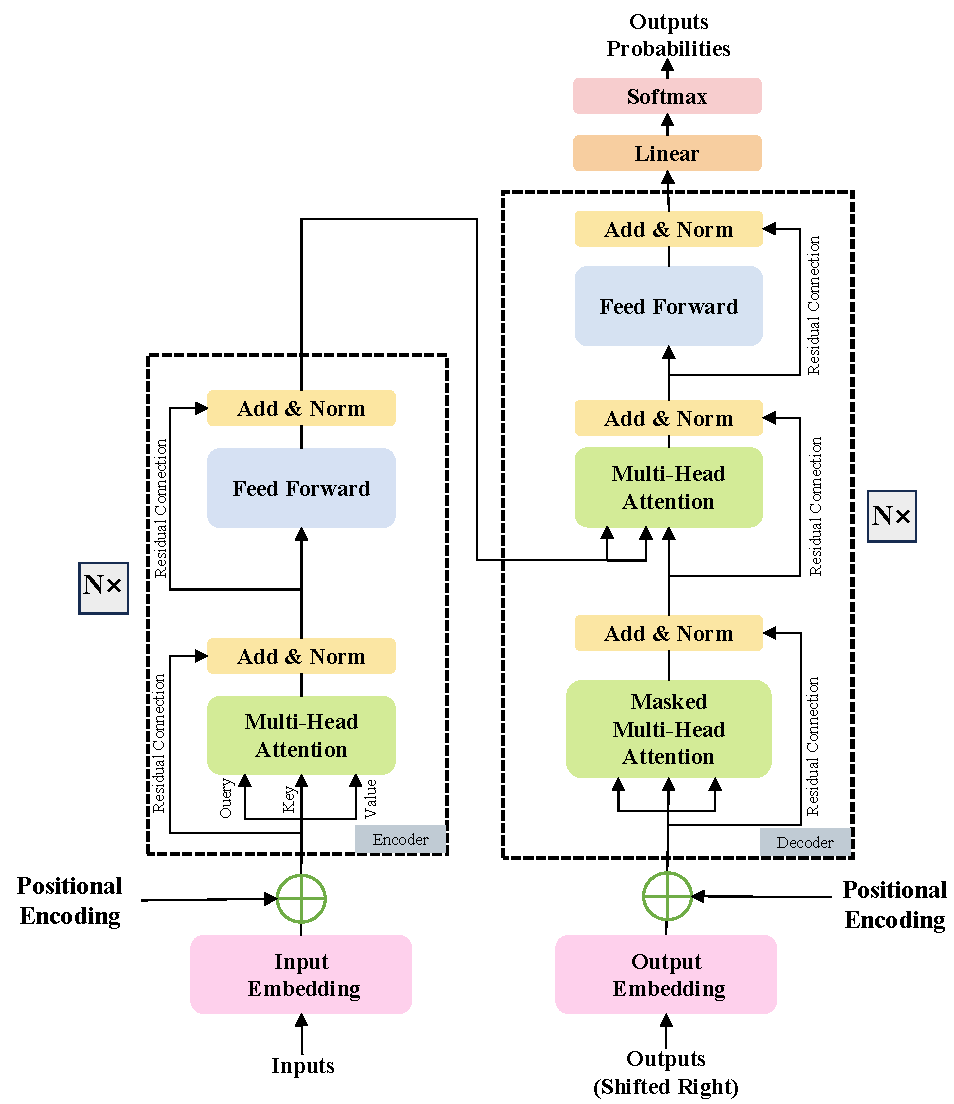
\includegraphics[width=0.5\textwidth]{trans.pdf}
\caption{Transformer Architecture (Vaswani et al. 2017). This architecture showcases a novel neural network design that relies heavily on self-attention mechanisms, removing the need for recurrence entirely. It consists of an encoder-decoder structure, where each is a stack of multiple identical layers. Attention scores are computed in the architecture to weigh input significance differently, enabling the model to focus on different parts of the input sequence when producing an output.}
\label{fig:one} % 图片的标签,用于引用
\end{figure}
%*************************************************************************************************%

The Transformer model can efficiently model and process sequence data by utilizing a self-attention mechanism, multi-head attention, and feed-forward neural networks, thereby achieving significant results in NMT tasks. The self-attention mechanism, a core component of the Transformer model, computes the association degree between each position in the input sequence and all other positions. This is done by applying these association degrees in a weighted sum to obtain the context representation of each position. This mechanism can be mathematically represented as follows:

\begin{equation}
\operatorname{Attention}(Q, K, V)=\operatorname{softmax}\left(\frac{Q K^T}{\sqrt{d_k}}\right) V
\end{equation}

Here, Q represents the query matrix, K represents the keys, V represents the values, and $d_k$ is the dimension of K.

The Transformer model introduces the concept of multi-head attention, which improves the model's capability to manage different types of information by concurrently computing multiple self-attentions. This can be represented as follows:


\begin{equation}
\operatorname{MultiHead}(Q, K, V)=\text { Concat }\left(\text { head }_1, \ldots, \text { head }_h\right) W_O
\end{equation}
%MultiHead(Q, K, V) = Concat(head_1,...,head_h)W_O

Where $head_i$ represents the computation result of the i-th attention head, $h$ is the number of attention heads, and $W_O$ is the output weight matrix.

In addition to the attention mechanisms, the Transformer employs a position-wise feed-forward network, which is applied to each position separately and identically. It consists of two linear transformations with a ReLU activation function in between:

\begin{equation}
\operatorname{FFN}(x)=\operatorname{ReLU}\left(x W_1+b_1\right) W_2+b_2
\end{equation}

Here, x represents the input, $W_1$ and $W_2$ represent the weight matrices of the two linear transformations, $b_1$ and $b_2$ represent the bias terms.

Please note that despite the impressive performance of the Transformer model on large-scale datasets, it often struggles in scenarios with scarce data. Researchers have proposed various strategies to address this issue, such as unsupervised training \cite{3-4}, data augmentation with monolingual corpora \cite{3-5}, or improving performance with knowledge distillation \cite{3-6}. These methods enhance the model's generalization ability, making the Transformer model more effective in low-resource language translation tasks.



%\indent The Transformer architecture has demonstrated remarkable success in modeling and processing sequence data, thanks to its innovative combination of self-attentive mechanisms, multi-headed attention, and feed-forward neural networks. This powerful combination allows the Transformer model to effectively capture global dependencies in a sequence, enabling it to focus on the most relevant parts of the input and generate high-quality outputs. As a result, the Transformer has achieved state-of-the-art results in various NLP tasks, particularly in NMT. \\
%\indent The self-attentive mechanism is a fundamental component of the Transformer architecture, and is used to calculate the degree of association between each position in the input sequence and other positions. This mechanism allows the model to capture global dependencies in the sequence, enabling it to effectively focus on the most relevant parts of the input and generate high-quality outputs.The self-attention formula used in the Transformer model is expressed as follows:
%%********************************公式1********************************************
%\begin{equation}
%\operatorname{Attention}(Q, K, V)=\operatorname{softmax}\left(\frac{Q K^T}{\sqrt{d_k}}\right) V
%\end{equation}
%%********************************公式1********************************************
%Q is the query matrix, K is the key value, V is the value, and $d_k$ is the vector dimension of K\\
%\indent Multi-headed attention is introduced in the Transformer model to enrich the expressive power of the model by computing multiple self-attentions in parallel.The multi-headed attention formula in the Transformer architecture is expressed as follows:
%%********************************公式2********************************************
%\begin{equation}
%\operatorname{MultiHead}(Q, K, V)=\text { Concat }\left(\text { head }_1, \ldots, \text { head }_h\right) W^O
%\end{equation}
%%********************************公式2********************************************
%$head_i$ represents the computation result of the i-th attention head, h denotes the number of attention heads, and $W^O$ represents the output weight matrix. \\
%\indent To further enhance the representational power of the Transformer architecture, a feed-forward neural network formulation is used to perform a nonlinear transformation of the contextual representation of each location. This enables the model to capture more complex and abstract relationships between different parts of the input sequence.The feed-forward neural network formulation can be divided into two parts: the linear transformation, the activation function and the second linear transformation:
%%********************************公式3********************************************
%\begin{equation}
%\operatorname{FFN}(x)=\operatorname{ReLU}\left(x W_1+b_1\right) W_2+b_2
%\end{equation}
%%********************************公式3********************************************
%x denotes the input, $W_1$, $W_2$ denote the weight matrices of the two linear transformations, $b_1$, $b_2$ denote the bias vectors of the two linear transformations, respectively\\

%\indent The Transformer model has demonstrated impressive results in natural language translation tasks, particularly in scenarios where data resources are scarce. As a deep learning model for self-supervised learning, the Transformer can be trained and optimized on large-scale datasets, enabling it to achieve high performance on translation tasks with abundant training data. For example, on the WMT14 English-German translation task, the Transformer model improved its performance by 2.0 BLEU scores over the best model at the time\cite{1-7}. However, in practical scenarios where parallel corpora are limited, even the Transformer model faces significant challenges. To address this issue, researchers have proposed several methods to utilize limited training datasets for model training. These methods include eliminating parallel data and using an unsupervised approach to train the NMT system\cite{3-4}, using a monolingual corpus to augment the training data\cite{3-5}, and using knowledge distillation to improve the performance of character-level neurolinguistic models\cite{3-6}. By leveraging these approaches, the Transformer model can improve its generalization ability and effectiveness, enabling it to achieve better performance in scarce resource translation tasks. This has the potential to greatly benefit a wide range of NLP applications, particularly in multilingual and cross-lingual scenarios where data resources are limited.

\subsection{Large Language Models }
%******************************************图2****************************************************%
%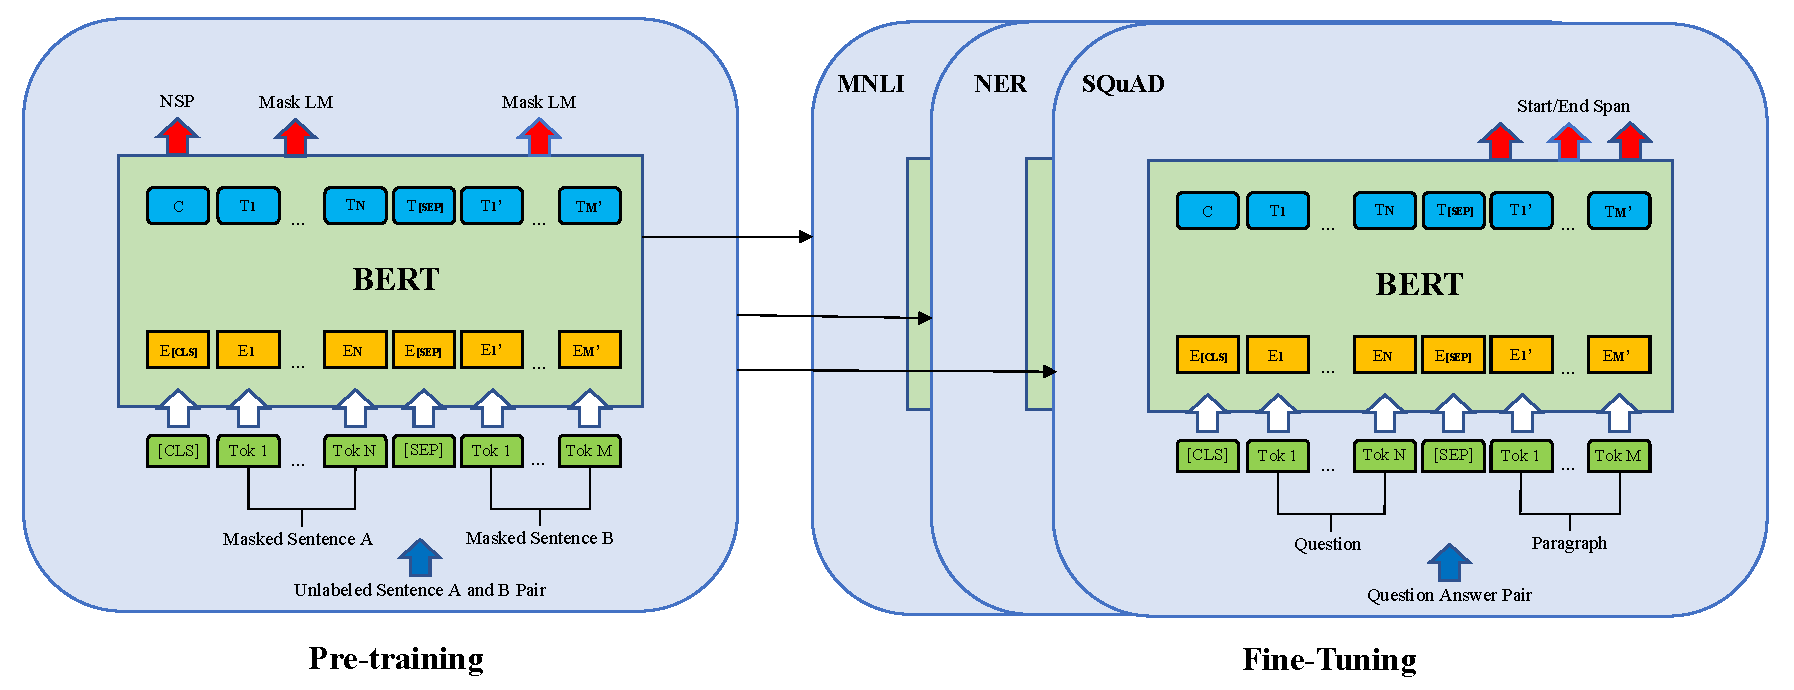
\includegraphics[width=0.72cm]{Bert.pdf}
%\caption{BERT architecture}

\begin{figure*}[htbp]
\centering
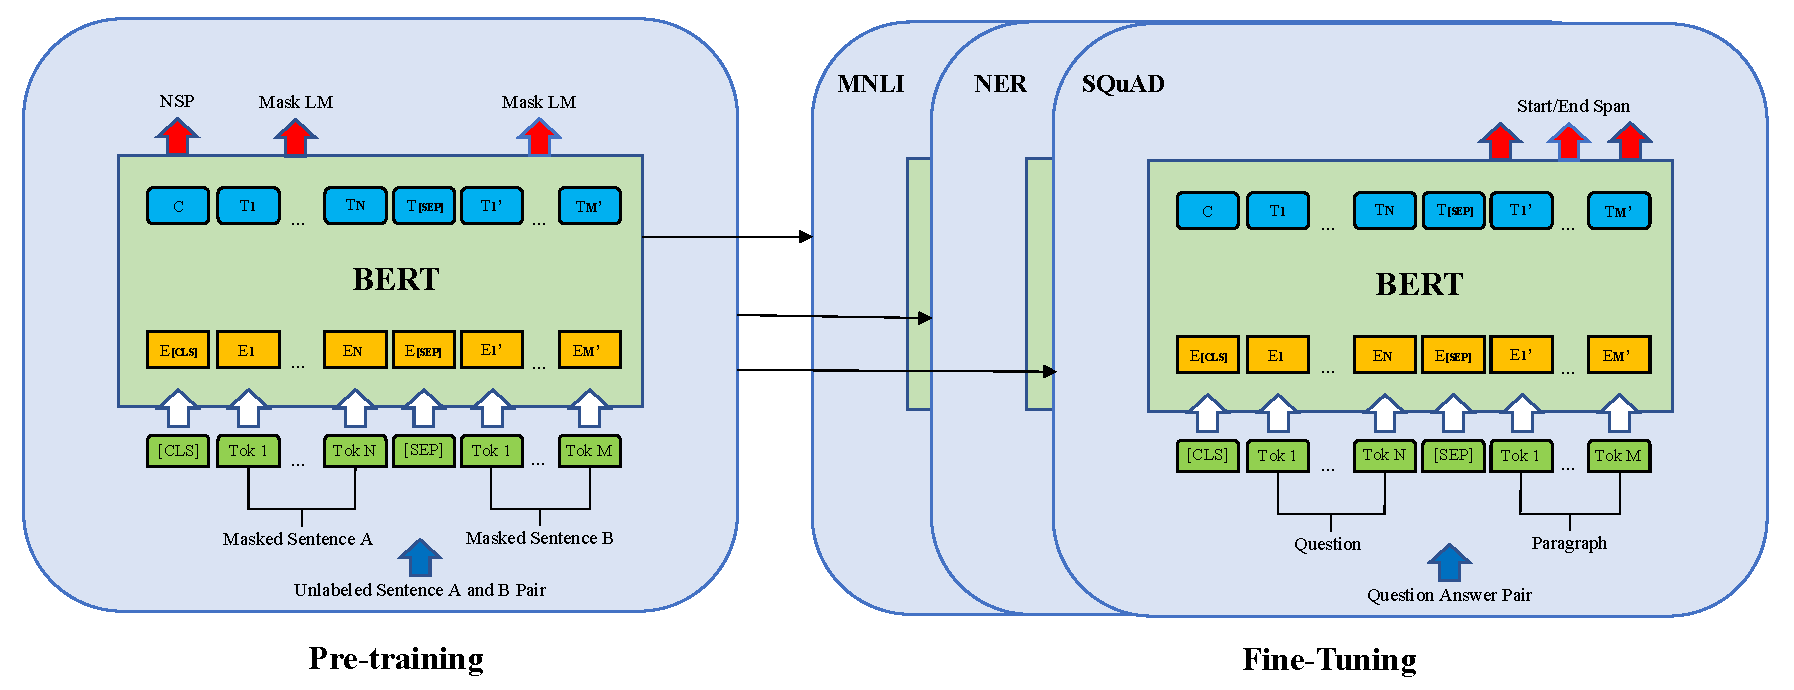
\includegraphics[width=1.0\textwidth]{Bert.pdf}
\caption{The comprehensive process of pre-training and fine-tuning in BERT (Devlin et al. 2018). Both phases utilize identical architectures with the exception of output layers. All downstream tasks are initialized using the same pre-trained model parameters. Throughout the fine-tuning phase, every parameter is adjusted. Special symbols, [CLS], are placed at the beginning of each input, while [SEP] acts as a distinct delimiter token, such as differentiating between questions and answers.}
\label{fig:two} 
\end{figure*}
%*************************************************************************************************%

LLMs played a pivotal role in the field of machine translation, leveraging their capacity to deeply comprehend contextual and semantic relations between source and target languages. This enhanced understanding significantly elevated the overall quality of translation. Through a combination of pre-training and fine-tuning, LLMs exhibited remarkable adaptability to diverse translation tasks, integrating both general language knowledge and specialized domain expertise. Furthermore, their proficiency in multi-language translation, context-awareness, and real-time translation facilitated meeting users' varied translation requirements, concurrently fostering continuous innovation and refinement in translation technology.

\color{red}


The Pre-trained Large Language Model (PLLM) is a language processing paradigm built upon the Transformer architecture, realized through extensive pre-training on vast text corpora. During this pre-training phase, the model develops an understanding of syntax, semantics, and the contextual nuances of language, empowering it to accurately predict missing words within a given context. BERT \cite{Jacob}, a prominent example of a PLLM based on the Transformer's encoder framework, was devised by Google to produce context-sensitive word embeddings, significantly advancing the efficacy of various NLP tasks. Distinguished from conventional language models, BERT incorporates bidirectional pre-training and employs a masking mechanism, as depicted in Fig. \ref{fig:two}.

The operational framework of BERT is segmented into two principal phases: pre-training and fine-tuning. The pre-training stage, illustrated on the left side of the figure, involves training BERT on a broad text corpus utilizing a multi-layered bidirectional Transformer encoder, which familiarizes the model with the statistical characteristics of the language. The fine-tuning stage, shown on the right, tailors the model to specific applications like SQuAD (Stanford Question Answering Dataset), NER (Named Entity Recognition), and MNLI (Multi-Genre Natural Language Inference) by refining it for particular tasks, thereby optimizing its performance.


Numerous scholars have explored the capabilities of BERT, with Zhang et al. \cite{Zhebin} introducing the BERT-JAM strategy to mitigate catastrophic forgetting during the fine-tuning process by progressively unfreezing model components. Further advancements, such as BiBERT \cite{Haoran}, RoBERTa \cite{Yinhan}, and ERNIE 2.0 \cite{Yu}, have continued to refine and expand upon BERT, significantly improving performance across a range of NMT tasks. Wu et al. \cite{Xueqing} utilized BERT for encoding contexts specific to translation tasks, aggregating all contextual sequences into a singular extended sequence for BERT encoding, thereby achieving superior translation outcomes. These developments underscore the transformative impact of PLLMs in enhancing the efficacy of natural language processing tasks.

Similar to BERT, BART (Bidirectional and Auto-Regressive Transformers) \cite{Mike}, rooted in the Transformer architecture for NLP and employing self-supervised learning, differs from BERT primarily in its modeling approach. BART is a sequence-to-sequence model that utilizes autoregressive and inverse generation tasks during pre-training, as opposed to BERT's MLM approach. This distinctive training methodology renders BART particularly adept for tasks in machine translation. La et al. \cite{Moreno} developed BART-IT, a variant of BART fine-tuned on an Italian text corpus and further refined on benchmark datasets for various summarization tasks. The study revealed that BART-IT outperformed other leading models, as evidenced by its ROUGE scores, highlighting the continuous evolution and application of PLLMs in advancing natural language understanding and processing.

Within the PLLM domain, following mBART, Laki et al. \cite{Laki} fine-tuned the mBART model with success in the English-Hungarian task. However, resource consumption remained high. Subsequently, Navarro et al. \cite{Navarro} enhanced the mBART model's performance by comparing it with state-of-the-art machine translation models in terms of user effort, WSR (Word Stroke Ratio), and MAR (Mouse Action Ratio) on a benchmark dataset in an interactive environment. Despite the experiments revealing limited performance in translating low-resource languages for pre-trained multilingual models like mBART, these models exhibited robustness to domain differences. Although their BLEU values remained below 3.0 for translations of unseen and typologically distant languages, Lee et al. \cite{Shiun} suggested a shift in focus from pursuing new models to exploring new data, underscoring the importance of data in this realm. In the pursuit of breaking language barriers, Meta's TEAM-NLLB developed the NLLB (No Language Left Behind) machine translation system \cite{Marta}, a conditional computing model aimed at bridging the performance gap between low- and high-resource languages, laying the groundwork for a universal translation system on a global scale.

ChatGPT \cite{OpenAI01} stood as a product of rapid technological development and continuous iterative updates in recent years. It represented the culmination of research in NLP, integrating underlying technologies such as Transformer, self-supervised learning, fine-tuning, human feedback reinforcement learning, and AI alignment \cite{Zhangqi}. LLMs like BLOOM \cite{Teven}, Falcon \cite{Ebtesam}, PaLM \cite{Aakanksh}, and the LLaMA family \cite{Hugo1} \cite{Hugo2} were also applied to translation tasks. In a related study, Zhu et al. \cite{Wenhao} compared the translation effects of numerous LLMs, highlighting features such as ``command semantics accidentally ignored'', ``cross-language examples more beneficial for low-resource translation'' and ``LLMs producing moderate translations on zero-resource languages''. Attention was drawn to the need for a shift from the pursuit of new models to the exploration of new data.

Prompt engineering assumed a significant role in assessing the translation capabilities of LLMs. Wu et al. \cite{Yangjian} trained the Lan-Bridge translation system based on GPT-3.5-16k for the WMT 2023 translation task in both English-to-Chinese and Chinese-to-English directions, using prompt technology to achieve optimal human evaluation results in document-level machine translation. Zhang et al. \cite{Biao} explored the feasibility of utilizing monolingual data and cross-language, cross-domain sentence-to-document conversion learning in prompting. They found that the quantity and quality of prompted examples significantly impacted translation outcomes. Jiao et al. \cite{Wenxiang} introduced the ParroT framework, leveraging open-source LLMs to enhance and regulate translation capabilities in chat. Experimental results indicated that translation instructions notably improved the original LLM's translation performance, emphasizing the importance of learning from low-quality translations labeled by humans. Ghazvininejad et al. \cite{Marjan} showcased LLMs' ability to address the rare word problem in machine translation through hints, particularly by providing control hints via bilingual dictionaries. The proposed DiPMT approach outperformed the baseline in both low-resource and domain-shifting machine translation. Li et al. \cite{Chunyou} proposed a multi-task machine translation (MT2) model that integrated multiple translation tasks, employing a context-specific learning cueing paradigm to significantly enhance the model's translation performance through a context-dependent training strategy.

In the realm of optimizing and fine-tuning LLMs, Yang et al. \cite{yang2023bigtranslate} introduced BigTranslate, expanding its coverage to over 100 languages by optimizing the LLaMA model. Preliminary experiments demonstrated that BigTranslate performed comparably to ChatGPT and Google Translate in multilingual translation. Notably, it even outperformed ChatGPT and Google Translate in eight language pairs. Zeng et al. \cite{DBLP:journals/corr/abs-2307-04408} proposed TIM, a 
novel framework leveraging preference loss to bootstrap LLMs for translation learning. Their approach outperformed existing methods on the WMT2022 test set, offering a fresh perspective on fine-tuning LLMs for translation tasks. Zhang et al. \cite{DBLP:journals/corr/abs-2306-10968} developed BayLing, aiming to transfer language generation and instruction-following capabilities from English to other languages through an interactive translation task. Experimental results indicated that BayLing performed on par with GPT-3.5-turbo in translation tasks but with a smaller parameter scale. Zhu et al. \cite{DBLP:journals/corr/abs-2308-04948} enhanced the performance of a pre-trained large language model on non-English languages through cross-language instruction fine-tuning and mixed use of multilingual resources, showcasing the advantages of cross-language models on various non-English benchmarks. Xu et al. \cite{DBLP:conf/nlpcc/XuWXH23} addressed the scarcity of bilingual data for low-resource machine translation by proposing a monolingual de-noising method using a large language model, significantly improving low-resource translation performance through fine-tuning the mBART model and error correction using ChatGPT. Xu et al. \cite{DBLP:journals/corr/abs-2309-11674} introduced ALMA, a novel fine-tuning method designed for translation tasks, achieving a significant improvement in machine translation performance through a two-stage fine-tuning strategy, surpassing existing LLMs.

Chain-of-Thought techniques proved effective for LLMs as well \cite{DBLP:conf/nips/Wei0SBIXCLZ22}. Zhao et al. \cite{DBLP:conf/acl/ZhaoLJQB23} proposed the Verify-and-Edit framework to enhance the factual correctness of text generated by LLMs. This framework improved factual accuracy by editing inference chains. Lu et al. \cite{DBLP:journals/corr/abs-2305-06575} introduced the Chain-of-Dictionary approach, enhancing machine translation performance by providing input words for a subset using a multilingual dictionary chain. This approach stimulated the translation ability of LLMs, particularly demonstrating a significant improvement in low-resource language translation.

Numerous studies delved into machine translation aspects related to LLMs. Lyu et al. \cite{DBLP:journals/corr/abs-2305-01181} explored emerging trends in machine translation using LLMs, discussing directions such as stylized translation and interactive translation, while emphasizing the importance of privacy preservation. Huang et al. \cite{DBLP:conf/nlpcc/HuangWLWSWYZ23} investigated an unsupervised framework for estimating machine translation quality using LLMs. By extracting sequence-level probability and uncertainty of LLMs as evidence for quality estimation, this framework achieved performance highly equivalent to human measures on the WMT 2022 test set. Fu et al. \cite{fu2024reasonableness} delved into the rationale behind the generalization of LLMs beyond machine translation capabilities. Their findings indicated that, even excluding the phenomenon of incidental sentence-level bilingualism in the training corpus, LLMs still exhibited impressive translation capability. They specifically examined the BLOOM family of models, highlighting the substantial contribution of unintentional bilingual alignment data at a finer granularity to the acquisition of translation capacity by language models. Bawden and Yvon \cite{DBLP:conf/eamt/BawdenY23} evaluated the large open-source multilingual model BLOOM in terms of machine translation performance, finding it performed well for multiple language pairs in a sample-less setting, despite challenges with zero-shot performance.

Various studies extensively explored GPT models' translation capabilities. Hendy et al. \cite{Amr}, Jiao et al. \cite{Wenxiang}, and Wang et al. \cite{Longyue} conducted detailed evaluations at both the sentence and document levels. Hendy et al. performed automated and manual evaluations, comparing ChatGPT with top-ranked translation systems on 18 language pairs and 4 domains in the WMT evaluation campaign. Jiao et al. conducted a preliminary study with ChatGPT for machine translation, revealing competitive performance in high-resource environments and suboptimal performance in low-resource environments or for remote language pairs. Following the release of GPT-4, improvements were observed in ChatGPT's performance for more distant languages. Wang et al. compared commercial MT systems and document-level NMT models with GPT models, focusing on discourse awareness evaluation. Human evaluation results indicated ChatGPT's superiority over commercial MT systems, offering promising avenues for document-level translation.

For LLMs' machine translation capability evaluation, Xu et al. \cite{xu} introduced InstructScore, an interpretable text generation evaluation metric combining explicit human instructions and implicit GPT-4 knowledge for fine-tuning. Lou et al. \cite{Lianzhang} proposed CCEval, a centralized multilingual machine translation evaluation benchmark dataset containing 2500 Chinese sentences translated into 11 languages, aiming to establish a high-quality evaluation standard. Additionally, studies \cite{Keqin} explored leveraging GPT models fully to optimize translation quality, addressing challenges through various cueing strategies or personalized MT. Robinson et al. \cite{Nathaniel} evaluated ChatGPT's machine translation performance across 204 languages, revealing competitive performance against or exceeding traditional machine translation on some high-resource languages but lagging on most low-resource languages, particularly underperforming on African languages.

While ChatGPT, based on the GPT model \cite{jiao2023chatgpt}, excelled in translating results for resource-rich Western languages, its performance lagged behind Google Translate, DeepL, and other models for low-resource languages. Zhu et al. \cite{Wenhao} systematically investigated the performance of LLMs and their challenges in multilingual machine translation, finding that although GPT-4 outperformed strongly supervised baselines in some translation directions, it still fell short of commercial translation systems, especially for low-resource languages. Table \ref{tab:A} illustrated the comparison between Chinese-centered and English-centered translation of GPT-4, revealing its suboptimal cross-language Chinese translation ability. Additionally, Table \ref{tab:B} serves as an example of prompts for this experiment.

%Additionally, the impact of the prompt on LLM translation ability was analyzed using XGLM-7.5B as an example in Table \ref{tab:B}, highlighting each prompt template's effect.

\begin{table}[htbp]
    \centering
    \caption{Performance of GPT-4 in English-centered as well as Chinese-centered translation (BLEU scores), the numbers following each language family indicate how many languages from that family are utilized.}
	\label{tab:A} 
    \begin{tabular}{lcccc}
        \toprule
        Language Family & X→Eng & X→Ch & Eng→X & Ch→X \\
        \midrule
        Indo-Euro-Germanic (8) & 48.51 & 27.97 & 40.64 & 24.13 \\
        Indo-Euro-Romance (8) & 47.29 & 27.31 & 44.47 & 27.12 \\
        Indo-Euro-Slavic (12) & 41.19 & 25.67 & 36.06 & 23.33 \\
        Indo-Euro-Indo-Aryan (10) & 37.30 & 21.81 & 21.35 & 13.55 \\
        Indo-Euro-Other (11) & 37.29 & 22.70 & 28.45 & 17.50 \\
        Austronesian (6) & 46.81 & 24.40 & 34.66 & 19.52 \\
        Atlantic-Congo (14) & 28.27 & 15.72 & 13.70 & 7.60 \\
        Afro-Asiatic (6) & 30.48 & 17.81 & 19.36 & 10.53 \\
        Turkic (5) & 31.73 & 19.96 & 20.96 & 14.02 \\
        Dravidian (4) & 33.10 & 20.63 & 18.60 & 11.37 \\
        Sino-Tibetan (3) & 27.74 & 20.88 & 22.81 & 16.30 \\
        Other (14) & 32.62 & 21.25 & 24.04 & 16.37 \\
        \bottomrule
    \end{tabular}

\end{table}


\begin{table}
    \centering
    \caption{Context learning is conducted using various templates with a fixed number of seven context examples. ``<X>'' and ``<Y>'' represent placeholders for the source and target sentences, respectively. ``[SRC]'' and ``[TGT]'' serve as placeholders for the source and target language, respectively.}
	\label{tab:B} 
    \begin{tabular}{>{\centering\arraybackslash}p{0.6\linewidth}>{\centering\arraybackslash}p{0.7\linewidth}}
        \toprule
        In-context Template  \\
        \midrule
        \texttt{<X> = <Y>} \\
        \texttt{<X> \textbackslash{}n Translate from [SRC] to [TGT]:\textbackslash{}n <Y>} \\
        \texttt{<X> \textbackslash{}n Translate to [TGT]: \textbackslash{}n <Y>}  \\
        \texttt{<X> \textbackslash{}n [TGT]: <Y>} \\
        \texttt{<X> is equivalent to <Y>}  \\
        \texttt{<X> \textbackslash{}n can be translated to \textbackslash{}n <Y>}  \\
        \texttt{[SRC]: <X> \textbackslash{}n [TGT]: <Y>}  \\
        \bottomrule
    \end{tabular}
\end{table}


%\begin{table}[htbp]
%    \centering
%    \caption{Context learning is conducted using various templates with a fixed number of eight context examples. "<X>" and "<Y>" represent placeholders for the source and target sentences, respectively. "[SRC]" and "[TGT]" serve as placeholders for the source and target language, respectively.}
%	\label{tab:B} 
%    \begin{tabular}{|l|}
%        \hline
%        \multicolumn{1}{|c|}{\textbf{In-context Template}} \\
%        \hline
%        \textbf{Reasonable Instructions:} \\
%        \hline
%        \begin{minipage}{0.8\textwidth}
%            \texttt{<X>=<Y>} \\
%            \texttt{<X> \textbackslash n Translate from [SRC] to [TGT]: \textbackslash n <Y>} \\
%            \texttt{<X> \textbackslash n Translate to [TGT]: \textbackslash n <Y>} \\
%            \texttt{<X> \textbackslash n [TGT]: <Y>} \\
%            \texttt{<X> is equivalent to <Y>} \\
%            \texttt{<X>\textbackslash n can be translated to\textbackslash n <Y>} \\
%            \texttt{[SRC]: <X> \textbackslash n [TGT]: <Y>}
%        \end{minipage} \\
%        \hline
%       
%    \end{tabular}
%\end{table}

Valdivieso and Arroyo's investigation \cite{sanz2023google} revealed that, despite ChatGPT making fewer errors in translating specialized terminology compared to Google Translate, professionals could not entirely rely on these machine translation tools. Karpinska and Iyyer \cite{Marzena} conducted a meticulous human evaluation of GPT-3.5 for literary passage translation. Their findings highlighted that while LLMs exhibited superior translation quality at the document level compared to standard sentence-level translations, critical errors were still prevalent, necessitating human translator intervention to preserve the author's original meaning.
\color{black}




%*****************************************4.稀缺资源自然语言机器翻译技术********************************************
%\subsection{\color{red}LLMs }
\section{Neural machine translation methods for low-resource languages}

\label{sec4}
Facing the challenges of low-resource language machine translation, scholars have actively explored various methods to enhance translation quality and efficiency. Among them, unsupervised/semi-supervised translation and data augmentation have become focal points of attention. This chapter will delve into these two key areas, dissecting their contributions to improving the performance of low-resource language translation.



\subsection{Unsupervised / Semi-Supervised Translation}

Unsupervised Neural Machine Translation (UNMT) has always been enhancing its ability to perform translations without parallel data. 
The main purpose of unsupervised learning is to discover hidden patterns and structures from unlabeled data, and the process is shown in Fig. \ref{fig:five}. Starting from the left, raw input data is fed into an algorithm, which is then processed through several steps: interpretation, model training, and further processing. The algorithm subsequently produces an output. Two key characteristics of this learning approach highlighted in the diagram are: first, the output is unknown; second, there is no predefined training dataset used in the process. This encapsulates the nature of unsupervised learning, which seeks patterns within input data without any prior labels or classes.
%******************************************图5****************************************************%
\begin{figure*}
\centering
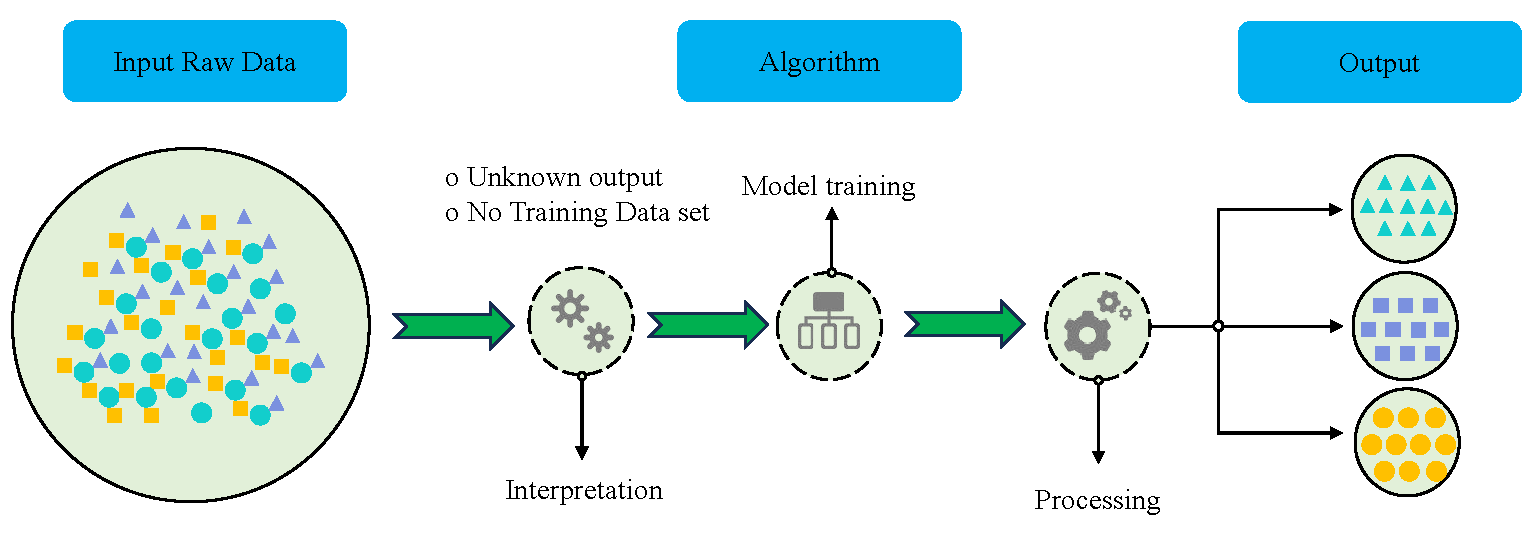
\includegraphics[width=0.7\textwidth]{UnsupervisedLearning.pdf} 
\caption{Flowchart of unsupervised learning. The diagram comprehensively depicts the entire process of unsupervised learning, from inputting raw data to producing output, traversing through various algorithmic steps, and notably, it operates without known outputs or a training dataset.} 
\label{fig:five} 
\end{figure*}
%******************************************图5****************************************************%

However, state-of-the-art methods often require a vast amount of monolingual data. To mitigate the problem of resource deficiency in the LR-NMT field, a novel effective method is proposed by Chronopoulou et al. \cite{n4-69}. They repurpose language models that have been pre-trained only on high-resource languages. The monolingual model is fine-tuned on both languages and is then used to initialize the UNMT model. A new method of lexical expansion is also introduced to accommodate new languages.

Edman et al. \cite{n4-70} observed that the unsupervised approach performs poorly in situations where monolingual data is limited, an issue stemming from the poor quality of pre-trained monolingual embeddings. By utilizing dependency-based word embeddings and restricting the monolingual data to one million sentences per language, they achieved a performance enhancement of about 1.5 BLEU points. They also found that the inclusion of subword information is pivotal to improving embedding quality.

In UNMT, the copy problem (i.e., direct copying of certain parts of the input sentences as translations) is quite common. Liu et al. \cite{n4-71} found this issue to be closely related to unexpected replication behaviors that occur in the online back-translation process. They proposed a simple yet effective training scheme, introducing a language discriminator loss to impose constraints on intermediate translations to generate the desired language. Through extensive experiments, including different types of language pairs, this method alleviates the replication problem and improves the translation performance for low-resource languages. 

Singh et al. \cite{n4-72} designed a UNMT system that uses a converter-based shared encoder and a language-specific decoder, trained by a denoising auto-encoder, and back-translated using multiple test references from the Manipuri side. The translation results of this system are promising. 

Sun et al. \cite{n4-73} introduced a simple method for translation among thirteen languages using a single encoder and a single decoder to enhance UNMT for all language pairs using multilingual data. 

The quality of pseudo-sentences in back-translation often impacts the quality of translation. In this context, Wu et al. \cite{n4-74} proposed a more effective alternative method to train an unsupervised translation system by extracting and editing real sentences from a target monolingual corpus and introducing a comparative translation loss for evaluation. Experiments show that this method consistently outperforms previous UNMT systems on low-resource language pairs, achieving a boost of up to 3.63 BLEU points.

Li et al. \cite{n4-75} introduced a novel reference language-based UNMT framework called RUNMT. In this framework, the reference language shares a parallel corpus with the source language. Despite the limited information source, the researchers introduced a reference agreement mechanism that uses the explicit signal provided by this corpus to assist in the reconstruction training of UNMT. This method improves the quality of UNMT compared to a strong baseline that uses only one auxiliary language.

Lample et al. \cite{n4-a1} explored how to learn translations with only a large-scale monolingual corpus at hand, proposing two model variants that leverage parameter initialization, language model denoising, and reverse translation to generate parallel data. These models perform exceptionally well in several benchmark tests, even outperforming existing methods on low-resource language pairs.

Conneau et al. \cite{n4-a2} demonstrated an unsupervised method to construct a bilingual lexicon between two languages by aligning the monolingual word vector space without using a parallel corpus. This method even surpasses existing supervised methods on cross-linguistic tasks for some language pairs and is applicable to long-distance language pairs. 

In the same year, Lample et al. \cite{n4-a3} investigated the possibility of learning translation without any parallel data. They proposed an unsupervised machine translation model by mapping sentences from two different languages into a shared latent space and learning to reconstruct both languages in this space. This approach represents a significant breakthrough in machine translation as it eliminates the need for labeled data, which is often expensive and time-consuming to obtain.

Dou et al. \cite{n4-76} proposed a method to improve the UNMT model by learning domain-aware feature embeddings, which significantly improves performance in multiple experimental settings. Simultaneously, it was discovered that combining this approach with back-translation could further enhance the model's performance.

Huang et al. \cite{n4-77} proposed a method to enhance unsupervised multimodal machine translation using visual content. Through multimodal back-translation and pseudo-visual rotation, a shared multilingual visual semantic embedding space was studied, and additional weak supervision was provided through captions. Experimental results showed that this model outperforms existing methods on the Multi30K dataset and has good generalization capabilities.


Xu et al. \cite{n4-78} proposed the Polygon-Net framework, which enhances the UNMT model by using multiple auxiliary languages. They design a new loss function and improve performance by sequentially updating and enhancing multiple unsupervised models. The framework significantly outperforms conventional methods on different datasets and performs better when more languages are introduced.

Semi-Supervised Neural Machine Translation (SNT) is a potent technique that utilizes a limited amount of bilingual data and a significant volume of unlabeled monolingual data for training. In SNT, labeled bilingual data are used for supervised training, while unlabeled monolingual data are deployed to enhance translation performance. The central idea behind SNT is to broaden the limited bilingual dataset by learning the correspondence between source and target languages with the help of unlabeled monolingual data. 

Nag et al. \cite{n4-79} proposed a semi-supervised NMT approach that leveraged a bilingual lexicon to improve model performance. They extended the model's lexicon and maintained high-quality content by generating word-by-word translated synthetic sentences. The experimental results indicated that this method achieved significant improvements over a robust baseline. 

Cheng\cite{n4-80} put forth a semi-supervised method for training an NMT model, which utilized a self-encoder and a translation model to process both labeled and unlabeled data. The self-encoder was used to reconstruct the monolingual corpus, and the translation model was applied as an encoder and decoder method. This system surpassed traditional methods on both Chinese and English datasets. 

Xu et al. \cite{n4-81} introduced a novel pairwise reconstruction objective to unify iterative back-translation and pairwise learning methods. This approach was found to enhance machine translation performance and effectively utilize the techniques of iterative back-translation and pairwise learning. 

Zhang et al. \cite{n4-82} employed a hierarchical coordination converter and a consistent pre-training converter to construct a translation model approach. Both models had different structures, yet identical parameters, ensuring consistency. The approach showed better performance with fewer parameters in low-resource situations in the experiments conducted. 

Wang et al. \cite{n4-83} proposed a method that explicitly exploited the connection of target monolingual data with source language data to aid NMT model training for monolingual data. The challenge of enumerating all possible candidate source sentences was avoided by employing a reverse translation model to sample potential source sentences. Then, two methods were proposed to leverage the law of total probability, including marginal distribution regularization and likelihood maximization for monolingual corpora. 

Kim et al. \cite{n4-84} discovered that linguistic differences and domain mismatches between source and target language data severely impacted performance, especially unsupervised learning in low-resource language pairs. The experiments demonstrated that supervised and semi-supervised baseline models outperformed the best unsupervised results on 50k sentences of bilingual data. 

\subsection{Augmentation of Training Data}

\subsubsection{Model Improvement}

Numerous studies have been conducted to improve translation models and provide translation support for low-resource languages. For instance, Mao et al. \cite{n4-1} proposed a Japanese-specific sequence-to-sequence model, named JASS (joint pre-training of BMASS and BRSS), which improved the translation quality in both Japanese-English and Japanese-Russian tasks. Xu et al.  \cite{n4-2} introduced a Dynamic Curriculum Learning (DCL) method for reordering the data. As DCL only modifies the training strategy and does not require any external data, it is of practical importance for real low-resource scenarios. The experimental results showed that this method can improve the level of translation. 
\color{green}Haddow et al. \cite{DBLP:journals/corr/abs-2109-00486} introduced various research methods on addressing low-resource machine translation, categorized into three main structures: data collection, data utilization, and model selection. The aim is to enhance both the quantity and quality of parallel and monolingual data available for low-resource machine translation, thereby optimizing the utilization of existing limited resources. Ranathunga et al. \cite{DBLP:journals/corr/abs-2106-15115} introduced a method for selecting the most suitable NMT techniques for low-resource language pairs. This approach takes into account the size and type of the dataset, as well as the available computational resources. They designed a flowchart for choosing the appropriate technology based on the given data specifications, aiming to enhance the translation quality. \color{black} Dou et al. \cite{n4-3} introduced a weighting strategy based on the current quality of sentences and their improvement relative to the previous iteration, enhancing the round-trip translation model. This was shown to be effective in the experimental results. Araabi et al. \cite{n4-4} improved translation on sparse resource languages by optimizing the translation model.

Addressing the challenge of rare word translation in low-resource language pairs, Ngo et al. \cite{n4-5} proposed two methods: one dynamically learns the similarity of tagged words in a shared space between source languages, and the other enhances the translation of rare words by updating the embeddings of rare words during training. The effectiveness of these methods was validated through experimental results.

In terms of data augmentation, Xia et al. \cite{n4-one1} proposed a framework for low-resource machine translation that centers on high-resource languages. It converts high-resource parallel data into low-resource data through a two-step rotation method. Experimental results indicated that this method effectively improves translation quality. 

Qin et al. \cite{n4-four4} proposed a data augmentation framework that generates multilingual code-switching data for fine-tuning mBERT. This framework encourages models to align the representations of the source language and multiple target languages at once by mixing contextual information. Experimental results showed that this method significantly improves performance on multiple language tasks.

Nguyen et al. \cite{n4-seven7} diversified the training data by using predictions from multiple forward and backward models and combining them with the original dataset, yielding good results on multiple translation tasks. Li et al. \cite{n4-eight8} proposed a novel data augmentation method that extends limited noisy data to further improve the robustness of the NMT model to noise, while maintaining model compactness. They also studied the effect of noise in external data on robustness, demonstrating its beneficial impact on improving robustness.

Kang et al. \cite{n4-nine9} presented a method that improves the performance of a character-decoder-based seq2seq model in extremely resource-limited situations through transfer learning and data augmentation. Chen et al. \cite{n4-ten10} investigated a data augmentation method for lexical constraint-aware NMT that constructs constraint-aware synthetic training data.

Duan et al. \cite{n4-eleven11} proposed a novel data augmentation strategy for NMT by considering the roles of words in sentences, setting sentence-specific selection probabilities, and using dependency parse trees as cues. Experimental results demonstrated a significant improvement in translation ability.

\subsubsection{Data Filtering}

Data filtering of training data has proven to be a successful technique in simultaneously improving the training efficiency and translation performance of Phrase-Based Machine Translation (PBMT). For instance, a data filtering technique proposed by Amittai et al. \cite{n4-6} has consistently shown excellent results, yielding significant gains for PBMT. Marlies et al. \cite{n4-7} introduced dynamic data selection techniques, with their progressive fine-tuning method obtaining good results on traditional static data selection and high-resource generalized baselines. In the field of NMT, Zhang et al. \cite{n4-8} also investigated data selection, proposing an active learning framework that selects informative source sentences to construct a parallel corpus, thereby minimizing the cost of human translation. 

For domain-specific translations, Wang et al. \cite{n4-9} conducted research on data selection and proposed a multi-domain balancing method for NMT to balance the domain distribution of training data, significantly enhancing the performance of NMT. Furthermore, Song et al. \cite{n4-10} improved data quality and translation accuracy by replacing the corresponding source language words with the target words in the target language. Li \cite{n4-11} proposed a method using XML tagging for a bilingual Chinese and Japanese parallel corpus, validating its effectiveness through experimentation. 

Without utilizing additional monolingual data, Li et al. \cite{n4-tow2} put forward a Diversity data augmentation method that extends training data by generating diverse pseudo-parallel data at both the source and target ends. Experimentation validated the effectiveness of this method. In a data augmentation method called SwitchOut, proposed by Wang et al. \cite{n4-five5}, words in the source and target sentences are randomly replaced with other random words in the corresponding vocabulary. Gao et al. \cite{n4-six6} presented a soft-context data augmentation method for NMT, which combines the contexts of multiple related words in the vocabulary and softly expands randomly selected words in the sentence. The effectiveness of the method was confirmed by experiments. 

Graça et al. \cite{n4-nineteen19} made improvements to the sampling approach and translation-generated synthetic data. Nishimura et al. \cite{n4-twenty20} proposed a data augmentation method for multi-source NMT that fills in incomplete parts of multi-source training data. Lastly, Sugiyama et al. \cite{n4-twentyone21} obtained a massively pseudo-parallel corpus by reverse-translating monolingual data, studying its effect on the translation accuracy of context-aware NMT models.

\subsubsection{Data Augmentation}

Back translation has been widely utilized for corpus augmentation in the field of machine translation. Sennrich et al. \cite{3-5} utilized back translation for corpus expansion, and this approach has since become a standard technique for data augmentation in machine translation. 
%******************************************************图3****************************************************%
\begin{figure}
\centering
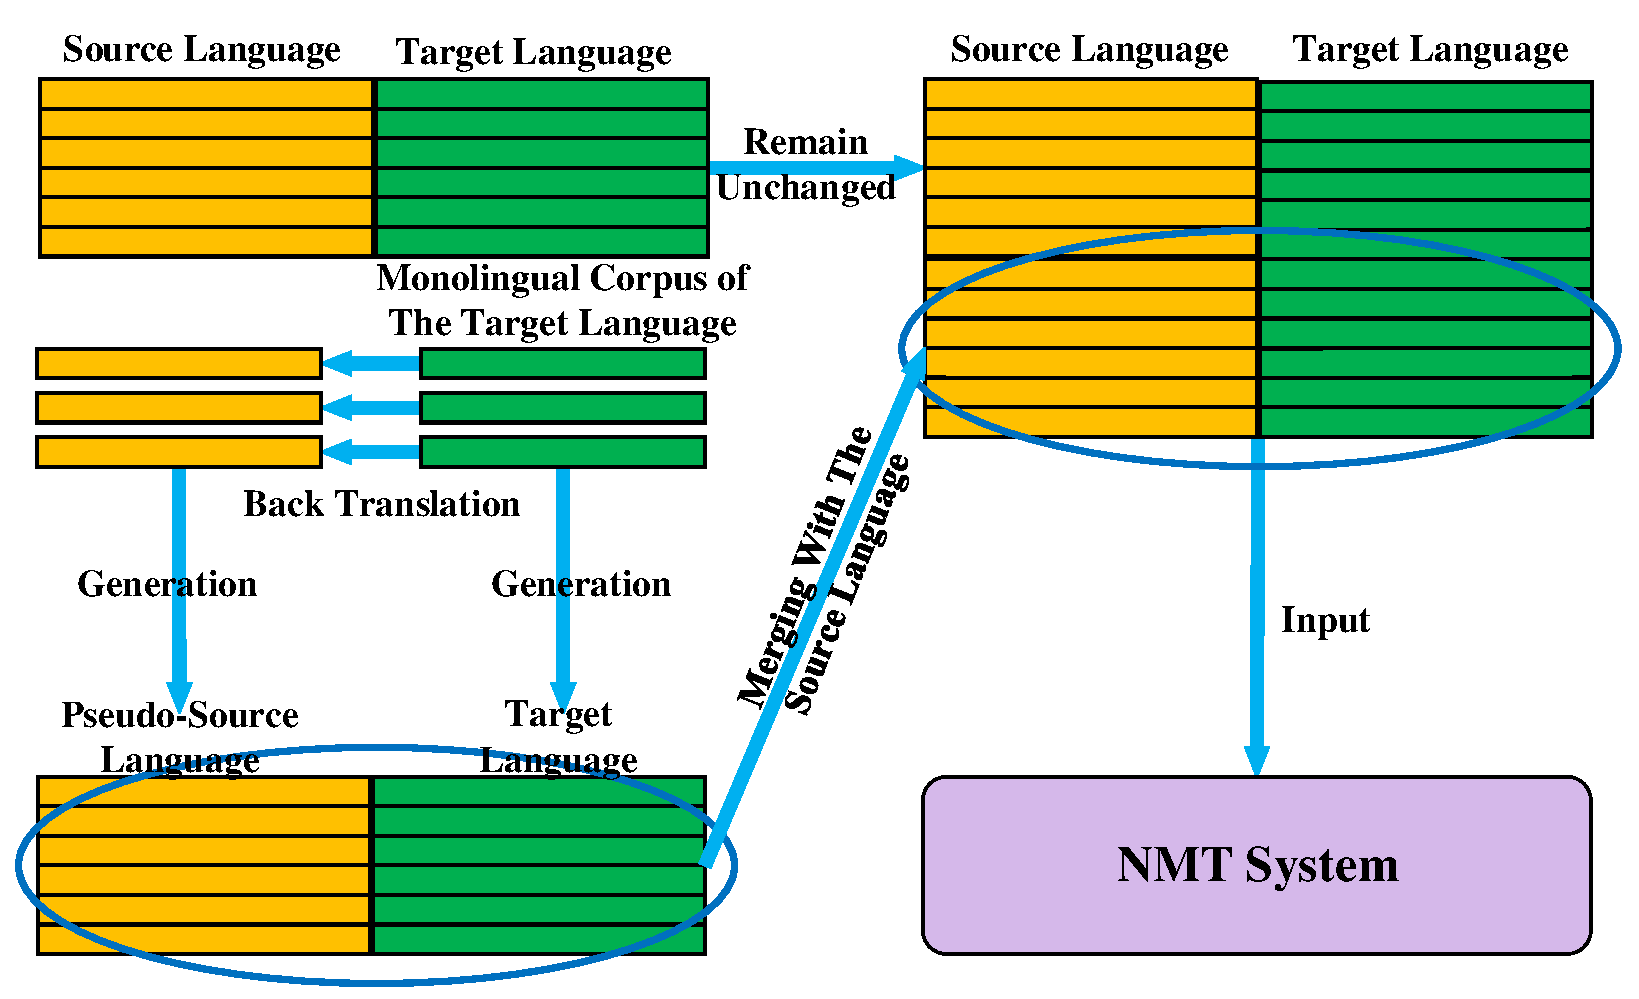
\includegraphics[width=0.8\textwidth]{Backtran.pdf} 
\caption{Flowchart of back-translation. The diagram provides a visual representation of the back-translation process. It highlights the progression from the source language (depicted in yellow) to the target language (in green). After back-translation, the pseudo-source language merges with the source language, reinforcing the origin corpus. This merged input is then fed into the NMT System, illustrating the full cycle of back-translation in NMT.} 
\label{fig:three} 
\end{figure}
%******************************************图3****************************************************%
As illustrated in Fig. \ref{fig:three}, the first step involves training a reverse translation model. This model is then used to translate the target language into the source language, generating pseudo source-language data. Finally, the augmented training set undergoes another round of training to achieve improved translation outcomes.


Compared to traditional noisy back translation, Caswell et al. \cite{n4-13} proposed TaggedBT, a method that offers a simpler and more stable alternative. During the back translation phase, Khatri et al. \cite{n4-14} weighted pseudo-parallel sentence pairs based on their quality, calculated using round-trip BLEU scores, consequently improving the performance of unsupervised NMT. 

Wei et al. \cite{n4-15} proposed a new iterative domain repair back-translation framework that introduces a Domain Repair model to refine the translation within synthetic bilingual data. Experimental results demonstrated significant improvement compared to unadjusted models and back-translation results. Abdulmumin et al. \cite{n4-16} proposed an iterative self-training approach to improve back translation by forward-transforming synthetic data generated using the backward model through multiple iterations to enhance its performance. This method proved superior to standard inverse translation and self-learning methods on English-German LR-NMT, according to experimental evidence. 

For back translation, Hieu et al. \cite{n4-17} proposed a dedicated meta-learning framework, which achieved good translation results. You et al. \cite{n4-18} put forward a data augmentation method based on the synonym substitution of low-frequency words, which achieved impressive results in Chinese-Vietnamese translation. Jia et al. \cite{n4-19} researched substitution based on larger granularity and proposed a phrase substitution-based method for generating Chinese-Vietnamese pseudo-parallel sentence pairs, effectively enhancing the performance of Chinese-Vietnamese NMT.


Recent years have seen a rise in collaborative machine translation projects between China and Japan, as presented by Zhao et al. \cite{n4-20}. This included discussions on cooperative backgrounds and foundations, intellectual property, specific cooperative content, and outcomes, as well as some reflections on the practical application of machine translation. Zhuang et al. \cite{n4-21} and Hagiwara et al. \cite{n4-22} integrated corpus data augmentation and chose the most recent model at the time for the IWSLT 2020 open domain translation task to establish relevant Chinese-Japanese NMT systems, respectively. 

Vaibhav et al. \cite{n4-twelve12} improved the robustness of machine translation systems by simulating naturally occurring noise in otherwise clean data. This noise includes spelling mistakes, slang, dialects, and personal language characteristics. By synthesizing this noise, the research could ultimately make conventional machine translation systems more resistant to naturally occurring noise, thereby alleviating to some degree the accuracy loss caused by it. Hassan et al. \cite{n4-thirteen13} proposed a method for generating training data that can transform a given parallel corpus of written and target languages into a parallel corpus of spoken dialect variants and the target language. The use of synthesized spoken data could improve the performance of large-scale translation systems. 

Inspired by computer vision work, Fadaee et al. \cite{4-2b5} proposed a new data augmentation method that targets low-frequency words by generating new sentence pairs containing rare words in new synthetic contexts. Experimental results under simulated low-resource settings have shown that this method yields effective performance gains.

Bulté et al. \cite{n4-fourteen14} devised a way to enhance the performance of NMT by utilizing the information in translation memory. This approach is easy to implement and promising for translation environments where sizable translation memory exists and there is some repetition of translation. Existing NMT data augmentation methods primarily rely on back translation, but issues arise from domain information differences leading to translation errors. Peng et al. \cite{n4-fifteen15} proposed a lexicon-based data augmentation method, which synthesizes a domain-specific lexicon and a generic domain corpus to generate a pseudo-IND parallel corpus, thus enhancing the benchmark model of the generic domain. 

Li et al. \cite{n4-sixteen16} proposed a data augmentation method using sentence boundary segmentation to improve the robustness of NMT to incoming ASR (Automatic Speech Recognition). Chinea-Ríos et al. \cite{n4-seventeen17} suggested a data augmentation method using the embedding representation of sentences to generate synthetic data. Finally, Li et al. \cite{n4-eighteen18} put forth a diversity data augmentation method for LR-NMT. By employing a restricted sampling strategy in the decoding process, they were able to generate different synthetic parallel data at the source and target.

\subsection{Zero-shot Translation}


Zero-shot translation leverages multilingual neural machine translation (MNMT) systems to perform translations between unseen language pairs. This ability to handle translations for pairs on which a model hasn't been explicitly trained is a distinguishing feature of zero-shot translation (ZST) and is underpinned by the model's capacity to learn language-agnostic representations. While the traditional multilingual NMT model often struggles to learn universal representations among different languages, leading to suboptimal zero-shot performance, pivot-based methods show promise in this arena \cite{10.1162/tacl_a_00065,ijcai2017p555}.

Numerous techniques have been developed to address the challenge of improving zero-shot translation performance. These can broadly be categorized into two: those that adjust the model's architecture to achieve universal representations \cite{lu-etal-2018-neural, JiZDZCL20, liu-etal-2021-improving-zero, chen-etal-2021-zero} and those that incorporate auxiliary training objectives to promote similarity across the representations of different languages \cite{abs-1903-07091, al-shedivat-parikh-2019-consistency, pham-etal-2019-improving, pan-etal-2021-contrastive}. 

Lu et al. \cite{lu-etal-2018-neural} introduced an NMT model that incorporates neural interlingua, enabling language-independent representations. This model facilitates direct zero-shot translation and allows for the classification of English Yelp reviews, which can be extended to classify French and German reviews. Despite having fewer parameters than multiple bilingual NMT models, their approach achieved comparable BLEU scores on the WMT15 dataset for each language pairing.

Ji et al. \cite{JiZDZCL20} highlighted the challenges faced by existing transfer methods in NMT during zero-shot translation due to language space discrepancies. To tackle this, they introduced an innovative transfer learning approach rooted in cross-lingual pre-training, ensuring all source languages occupy the same feature space. This involved utilizing one monolingual and two bilingual pre-training methods to establish a universal encoder for various languages. Experimental results demonstrated that their method surpasses the pivot-based baseline and several multilingual NMT strategies.

Liu et al. \cite{liu-etal-2021-improving-zero} addressed the challenges in MNMT, particularly in zero-shot translation, which often underperforms. They identified the positional correspondence to input tokens as a primary cause and proposed removing residual connections in an encoder layer, resulting in substantial gains in zero-shot translation quality.

Chen et al. \cite{chen-etal-2021-zero} explored the potential of using a multilingual pre-trained encoder (MPE) to enhance the cross-lingual transferability of NMT models, a topic previously under-investigated. They introduced SixT, a model that leverages MPE and employs a two-stage training schedule, enhanced by a position-disentangled encoder and a capacity-boosted decoder. Remarkably, Sixt surpassed existing models, including mBART, in zero-shot any-to-English tests, even with reduced training data and computational costs.

Arivazhagan et al. \cite{abs-1903-07091} investigated the challenges multilingual NMT models face in zero-shot translation, pinpointing failures in models reliant solely on parameter sharing. They introduced auxiliary losses for the NMT encoder to ensure consistent representation across languages, which significantly elevated zero-shot translation results without compromising supervised tasks. Notably, their method achieved competitive zero-shot performance on WMT14 English-French-German, matching the results of pivoting strategies.

Al-Shedivat et al. \cite{al-shedivat-parikh-2019-consistency} delved into the challenges of zero-shot generalization in multilingual translation, emphasizing the impact of available parallel data on its efficiency. They reframed multilingual translation as probabilistic inference, pinpointed why standard training methodologies falter in zero-shot tasks, and then proposed a consistent agreement-based training method that aligns translations across auxiliary languages. Their approach led to a 2-3 BLEU score improvement in zero-shot translation on various benchmarks without compromising the quality of supervised translations.

Pham et al. \cite{pham-etal-2019-improving} examined the zero-shot translation capabilities of multilingual NMT models, aiming to better understand inter-language information capture. They designed an encoder architecture independent of the source language, leading to insights on multilingual representation learning, and developed regularization methods to enhance the Transformer model's robustness in zero-shot scenarios. Their approach yielded a 2.23 BLEU point increase across 12 language pairs on the IWSLT 2017 dataset, confirming its effectiveness even for pairs with multiple intermediate pivots.

Pan et al. \cite{pan-etal-2021-contrastive} addressed the gap in non-English multilingual machine translation by introducing mRASP2, a unified training method aimed at achieving a universal cross-language representation. Leveraging a contrastive learning scheme and data augmentation, their approach significantly enhanced token alignment across languages. The method surpassed the performance of existing models for English-centric translations and yielded an average improvement of over 10 BLEU points for non-English directions compared to the multilingual Transformer baseline.

In particular, Gu et al. \cite{gu-feng-2022-improving} proposed an agreement-based training method to assist the MNMT model in generating consistent translations for semantically equivalent sentences. However, many of these methods, despite their potential, are not widespread due to issues like reduced supervised translation performance, complex algorithmic implementations, and intricate hyperparameter optimization.

Past research has also explored various innovations like using language tags \cite{wu-etal-2021-language}, introducing residual connections \cite{liu-etal-2021-improving-zero}, and devising novel training objectives \cite{al-shedivat-parikh-2019-consistency, pham-etal-2019-improving, abs-1903-07091, gu-etal-2019-improved, zhu-etal-2020-language, zhang-etal-2020-improving, wang-etal-2021-rethinking-zero} to bolster ZST effectiveness.


\section{Neural machine translation techniques for low-resource languages}


\subsection{Transfer Learning}

In recent years, Transfer Learning (TL) has been widely applied in low-resource languages. Transfer learning methods in NMT often involve initializing a low-resource model (child model) with a high-resource model (parent model).  TL leverages the knowledge and parameters of pre-trained models to enhance translation model performance. Pre-trained language models or translation models can be used as a foundation, and strategies such as feature extraction, joint training, or fine-tuning can then be employed to migrate the knowledge from the pre-trained models to the target task. In addition, data augmentation and filtering can enhance data quality and diversity. Transfer learning in NMT can improve the model's generalization capability and adaptability, thereby improving translation quality. The transfer learning process is illustrated in Fig. \ref{fig:four}. It highlights the process of acquiring knowledge from a source task/domain using a model, and then applying this knowledge to a different but related target task/domain via a refined model. The essence of this process is leveraging the understanding gained from one problem to solve a related issue more efficiently.

%******************************************图4****************************************************%
\begin{figure}
\centering
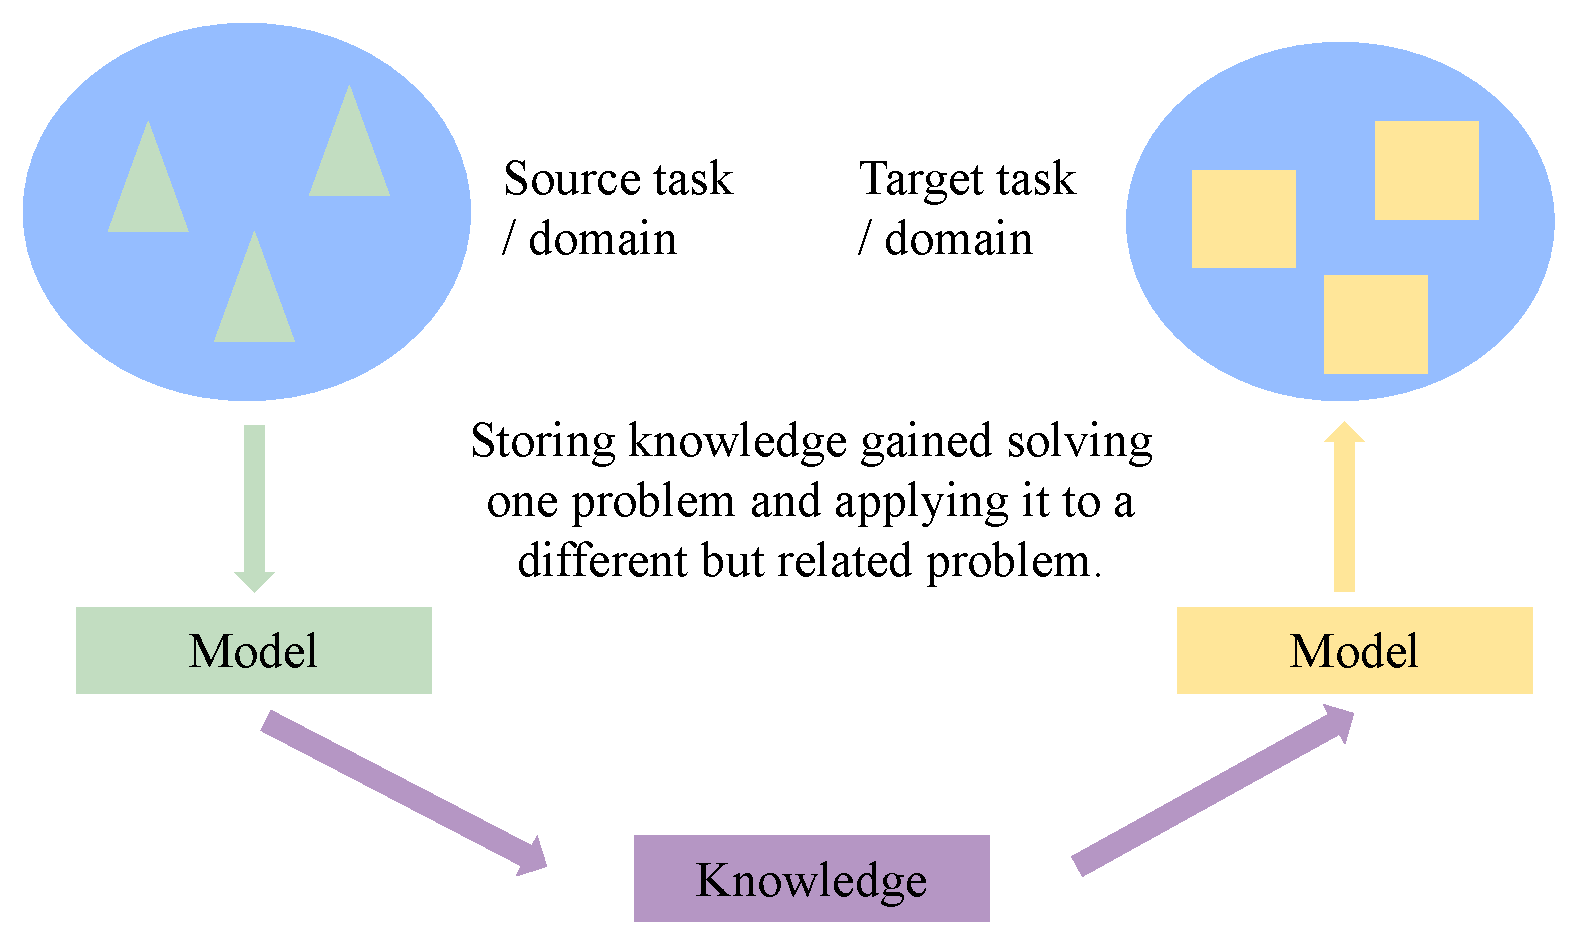
\includegraphics[width=0.65\textwidth]{Transferlearning.pdf} 
\caption{Flowchart of transfer learning. This diagram illustrates the process of transfer learning, detailing how knowledge is stored from a source task or domain and then applied to a target task or domain.} 
\label{fig:four} 
\end{figure}
%******************************************图4****************************************************%


Maimaiti et al. proposed a language-independent and direct Multi-Round Transfer Learning approach for LR-NMT\cite{n4-57}. To mitigate character-level differences between high-resource and low-resource languages, they introduced a unified phonetic translation method for language families with highly similar semantics and syntax. The approach led to an improvement of 5.63 BLEU scores. 

Inspired by human transfer reasoning and learning capabilities, Luo et al. \cite{n4-58} developed a new low-resource language-level transfer learning system to fully leverage valuable linguistic data. Meanwhile, Kim et al. \cite{n4-59} proposed a pre-training strategy using parallel corpora involving central languages, notably source-center, and center-target, leading to significant improvements in source-target translation.

Aji et al. \cite{n4-60} conducted studies demonstrating the importance of word embeddings in transfer learning, particularly when correctly aligned. They found that transferring only word embeddings without the rest of the content led to subpar results. Dabre et al. \cite{n4-61} empirically confirmed the impressive utility of multi-parallel corpora for transfer learning in a one-to-many LR-NMT setting.

While most State-Of-The-Art NMT systems achieve satisfactory results based on high-resource parallel corpora, the translation quality for low-languages remains suboptimal. To address this issue, Maimaiti et al. \cite{n4-62} proposed a hybrid transfer learning method for unrelated languages that leverages shared lexical embeddings without resorting to back translation or manual noise injection. The approach starts by training a parent model for high-resource languages and its lexicon, then employs an oversampling method to combine parent and child language pairs to train a hybrid model, followed by fine-tuning the child model. 

Imankulova et al. \cite{n4-63} proposed a novel multilingual multi-stage fine-tuning method that exploits out-of-domain data through transfer learning. This method involves first training a multilingual NMT model, then fine-tuning it using domain-parallel and back-translated pseudo-parallel data across multiple stages. This method led to an improvement of 3.7 BLEU scores.

Ji et al. \cite{JiZDZCL20} proposed an effective transfer learning method based on cross-language pre-training. The key idea is to enable all source languages to share the same feature space, allowing for a smooth transition to zero-shot translation. The researchers introduced one monolingual and two bilingual pre-training methods to create a universal encoder applicable to different languages. This method surpassed other NMT methods in experiments.

Xing et al. \cite{n4-65} enhanced Parent-Child transfer learning-based NMT with a bidirectional adaptive learning strategy. The internal components of the Parent encoder are divided into T1 and T2 teams. T1 encodes low-resource languages in a bilingual shareable potential space, while T2 directly transfers to low-resource languages.

Li et al. \cite{n4-66} proposed a new method named ConsistenTL, which continuously migrates knowledge from the parent model during the child model's training. This approach equates to the child model learning each instance under the guidance of the parent model. ConsistenTL led to significant improvement over the strong transfer learning baseline with a gain of up to 1.7 BLEU scores.

Building upon the mainstream transfer learning architecture, Luo et al. \cite{n4-67} proposed a new approach that perfectly integrates back translation with NMT model initialization. This method not only initializes the NMT model by transferring the parameters of the pre-trained model but also generates synthetic parallel data by translating large-scale monolingual data from the target side to improve translation fluency. Finally, Goyal et al. \cite{n4-68} proposed a multilingual transfer learning technique that utilizes parallel data from multiple related languages to aid in the translation of low-resource language pairs.






%
%Unsupervised Neural Machine Translation (UNMT) has achieved remarkable progress in recent years, but state-of-the-art methods often require a large amount of monolingual data. 
%The main purpose of unsupervised learning is to discover hidden patterns and structures from unlabeled data, and the process is shown in Figure 5, which is roughly divided into four steps: data collection, feature extraction, model training, and result processing.
%%******************************************图5****************************************************%
%\begin{figure*}
%\centering
%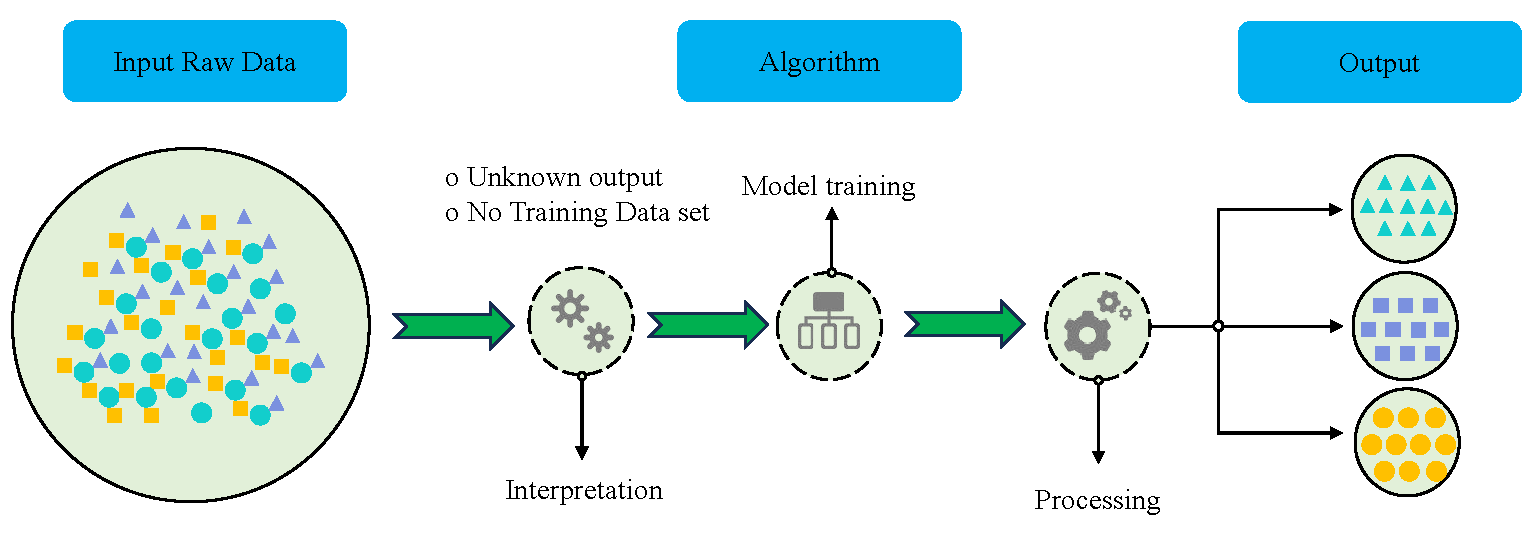
\includegraphics[width=0.7\textwidth]{UnsupervisedLearning.pdf} 
%\caption{Flowchart of Unsupervised Learning} 
%\label{fig:five} 
%\end{figure*}
%%******************************************图5****************************************************%
%
%To address this issue in the Low-Resource Neural Machine Translation (LRNMT) domain, Chronopoulou et al\cite{n4-69}. propose a novel method that reuses pre-trained language models on high-resource languages. The monolingual model is fine-tuned on both languages and then used to initialize the UNMT model. A new lexical extension method is also introduced to accommodate new languages.
%Edman et al\cite{n4-70}. find that the UNMT method performs poorly with limited monolingual data, stemming from the low quality of pre-trained monolingual embeddings. By using dependency-based word embeddings and limiting the monolingual data to 1 million sentences per language, the researchers achieve a performance improvement of about 1.5 BLEU scores. The inclusion of subword information is found to be crucial for improving embedding quality and addressing the "copy problem," where some parts of the input sentences are directly copied as translations.
%Liu et al\cite{n4-71}. propose a simple yet effective training scheme that introduces a language discriminator loss to impose constraints on intermediate translations to generate the desired language, thus alleviating the replication problem and improving translation performance for low-resource languages.
%Singh et al\cite{n4-72}. design a UNMT system that uses a converter-based shared encoder and a language-specific decoder, trained by a denoising auto-encoder, and back-translated using a Manipuri-side multiple test reference. The translation results of this system are encouraging.
%Sun et al\cite{n4-73}. introduce a simple method for translation between 13 languages using a single encoder and a single decoder to improve UNMT for all language pairs using multilingual data.
%Wu et al\cite{n4-74}. propose a more effective alternative method to train an unsupervised translation system by extracting and editing real sentences from a target monolingual corpus and introducing comparative translation loss for evaluation. Experiments demonstrate that this method consistently outperforms previous UNMT systems on low-resource language pairs, achieving a boost of up to 3.63 BLEU scores.
%Li et al\cite{n4-75}. propose a novel reference language-based UNMT framework called RUNMT, which uses a reference language that shares a parallel corpus with the source language and an explicit signal provided by this corpus to assist the reconstruction training of UNMT.
%Lample et al\cite{n4-a1}. explore how to learn translations with only a large-scale monolingual corpus, proposing two model variants that utilize parameter initialization, language model denoising, and reverse translation to generate parallel data. These models outperform existing methods on resource-scarce language pairs.
%Conneau et al\cite{n4-a2}. demonstrate an unsupervised approach to construct a bilingual lexicon between two languages by aligning the monolingual word vector space without using a parallel corpus. This method surpasses existing supervised methods on cross-linguistic tasks for some language pairs and is applicable to long-distance language pairs.
%In the same year, Lample et al\cite{n4-a3}. investigated the possibility of learning translation without any parallel data. They proposed an unsupervised machine translation model by mapping sentences from two different languages into a shared latent space and learning to reconstruct both languages in this space. This approach represents a significant breakthrough in machine translation, as it eliminates the need for labeled data, which is often expensive and time-consuming to obtain.
%Dou et al\cite{n4-76}. propose a method to improve the UNMT model by learning domain-aware feature embeddings, which significantly improves performance in multiple experimental settings. Huang et al\cite{n4-77}. propose a method to improve unsupervised multimodal machine translation using visual content, which outperforms existing methods on the Multi30K dataset and has good generalization capability. Finally, Xu et al\cite{n4-78}. propose the Polygon-Net framework, which enhances the UNMT model by using multiple auxiliary languages and updating and enhancing multiple unsupervised models.
%\\
%\indent The main purpose of unsupervised learning is to discover hidden patterns and structures from unlabeled data, and the process is shown in Figure 5, which is roughly divided into four steps: data collection, feature extraction, model training, and result processing:
%%******************************************图5****************************************************%
%\begin{figure*}
%\centering
%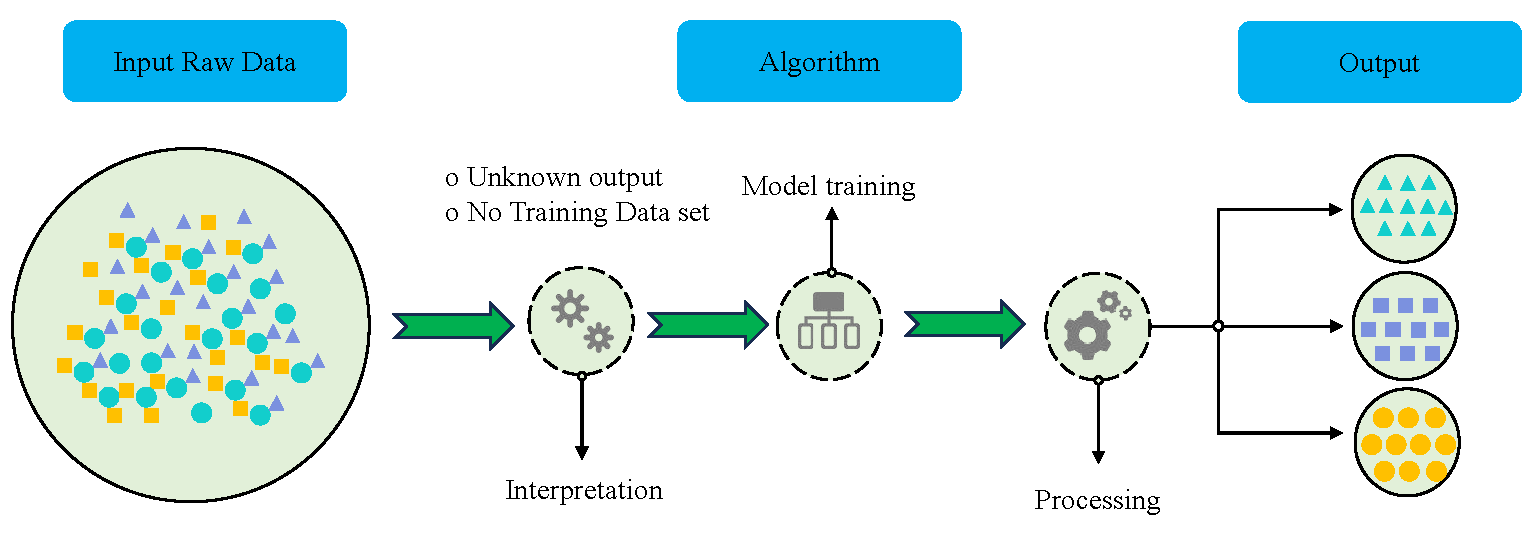
\includegraphics[width=0.7\textwidth]{UnsupervisedLearning.pdf} 
%\caption{Flowchart of Unsupervised Learning} 
%\label{fig:five} 
%\end{figure*}
%******************************************图5****************************************************%





\subsection{Improvements in Translation Models}

\subsubsection{Advancements in the Structure of the Transformer Model}

The Transformer model has become the mainstream model in machine translation tasks due to its excellent performance in multilingual translation experiments. Addressing limitations in the Transformer model, such as the requirement for predetermined input length and incoherent text semantic context, Dai et al. \cite{n4-23} proposed the Transformer-XL model, which improves long-term relationship limitations. To alleviate the complexity inherent to the standard Transformer model structure, Zhao et al. \cite{n4-24} put forth a simplification scheme based on a sparse mechanism, enhancing the focus of the Transformer model's attention. In an effort to resolve constraints on the attention mechanism and sequence context discontinuity, Beltagy et al. \cite{n4-25} introduced the Longformer model. This model adopts three strategies: windowing, receptive field expansion, and computation of a global attention representation sequence. Zaheer et al. \cite{n4-26} proposed a mechanism named Big Bird, which also leverages a sparse attention mechanism to reduce computational complexity to linear. The proposed mechanism mainly includes random, local, and global attention and effectively improves the performance of deep neural networks. 

For Long Short-Term Forecasting, Zhou et al. \cite{n4-27} designed an efficient model based on the Transformer, named ``Informer''. Informer addresses issues of long sequence prediction inherent to the Transformer, such as time complexity, memory occupation, and codec limitations. They introduced tools like the ProbSparse attention mechanism, self-attention distillation technique, and generative decoder to alleviate and resolve these problems, resulting in promising prediction outcomes.

Various methods for improving the NMT model were also suggested by other researchers. Song et al. \cite{n4-28} proposed an improvement method for NMT models focusing on Russian suffix translation. Xiao et al. \cite{n4-29} presented an interactive machine translation method based on a bilingual text-filling task. By pushing the depth of the Transformer up to 1000 layers, Wang et al. \cite{n4-30} were successful in enhancing the training stability of the model, improving the BLEU scores by 5\% compared to the Meat AI's M2M model. Zhang et al\cite{n4-31}. proposed a frequency-aware token-level contrast learning method. In this method, each decoding step's hidden state uses a soft contrast learning method based on corresponding word frequency to avoid confusion with correspondences to other target words. This not only significantly improves translation quality but also enhances lexical diversity and optimizes the word representation space. 

To enhance the performance of the NMT model. \color{green} Li et al. \cite{DBLP:journals/corr/abs-2204-04344} presented the champion system for a low-resource multilingual translation task centered around Chinese in the 2021 iFlytek AI Developer Competition. The system utilized techniques such as monolingual word embedding data augmentation, bilingual curriculum learning, and contrastive re-ranking. They introduced a novel In-trust loss function to replace the traditional cross-entropy loss, resulting in improved translation performance. The results demonstrated that the implementation of these ideas outperformed other state-of-the-art methods, including the mBART model, M2M model, and Google Translate engine experiments. \color{black}Wang et al. \cite{n4-32} introduced two KNN (K-Nearest-Neighbor) modules. One is used to memorize correct sentence feedback provided by humans, and the other adaptively balances the use of historical human feedback and the original NMT model. Building upon this, they proposed a nonparametric online learning method that does not require changes to the original model structure.

\subsubsection{Model Improvements Based on Language Characteristics}

According to the research by Meng et al. \cite{n4-33}, the optimal choice for Chinese NLP-related tasks is to use models trained at the character level. The research conducted by Cherry and his team \cite{n4-34} indicates that for character-level translation models, the standard sequence-to-sequence architecture of sufficient depth can effectively address the problem of character-level modeling. Moreover, deep models operating at the character level outperform their counterparts running on word fragments. 

Ataman et al. \cite{n4-35} designed a hierarchical decoding architecture, which provides a more efficient character-level scheme, thereby conserving computational resources. 
Chen and his team \cite{n4-36} improved the translation model by incorporating a multi-layer granularity approach. 

Zhang et al. \cite{n4-37} proposed a simple yet effective subcharacter-level Chinese translation method that utilizes the Five Strokes (Wubi) input method. 
Currey et al. \cite{n4-38} leveraged linearized parsing of source training sentences to inject syntactic parsing information into the Transformer architecture, without modifying it. While this approach performs well on language pairs with low-resources, it could potentially lead to a drop in quality when applied to resource-rich language pairs. 

Gao et al. \cite{n4-39} explored the potential applicability of self-attentive models in character-level NMT. Ma et al. \cite{n4-40} concluded through comprehensive metric evaluations and manual examination experiments that character-level implementations show promising performance.

Finally, Luo et al. proposed a model tuning method for Chinese-Japanese NMT \cite{4-2-12}.




\subsection{Integration of External Knowledge}

The integration of pre-prepared external knowledge such as monolingual, bilingual, and annotated data can not only guide the learning process of NMT but can also enhance its interpretability.

\subsubsection{Fusion of Alignment Information}

Li et al. \cite{n4-42} proposed two methods for acquiring alignment information, independent of the attention mechanism. The EAM (Explicit Alignment Model) necessitates a large weight matrix W, which computes the probability of a source word corresponding to the target word. As the W matrix is large, it requires substantial annotated alignment data, which can be auto-generated by fast\_align. Another method, termed Prediction Difference, substitutes the word vector of words in the source sentence with a 0 vector and observes the change in predicted probability. These methods have proven to improve the alignment success rate for high-contribution words from the source sentence, thereby enhancing machine translation quality.

Xiang et al. \cite{n4-43} used statistical alignment methods to model structural differences between the Chinese and Vietnamese languages, thereby extracting linguistic feature differences between them, which improved the quality assessment of Chinese to Vietnamese translations. Song et al. \cite{n4-44} proposed an NMT framework that incorporates alignment information.

\subsubsection{Integration of Syntactic Knowledge}

Integration of more linguistic information into NMT models can be achieved through encoders and decoders. Sennrich et al. \cite{n4-45} proposed a feature combination encoder that integrates various feature vectors including word root features, subword tagging features, morphological features, lexical annotations, and dependency tagging features. Additionally, Chen et al. \cite{n4-46} extended the encoder and decoder structures and fused more linguistic features, such as dependency features, to improve the representation of the source language and generation of the target language. 

Eriguchi et al. \cite{n4-47} introduced a tree-to-sequence NMT model that uses a syntactic tree-based encoder to capture phrase structural information of source language sentences from the bottom up. 
Chen et al. \cite{n4-48} advanced this approach by proposing a bidirectional syntactic tree encoder that can integrate both sequential and tree-based representations of the language. 

Gū et al. \cite{n4-49} developed a novel syntactic tree structure model that combines the encoder with a perception-enhanced syntactic tree structure. 
Pham et al. \cite{n4-50} revealed that the Transformer model can effortlessly capture syntactic structures, but the same translation results can be achieved even if a linear tree is used instead of actual dependencies. 

Chang et al. \cite{n4-51} researched encoders for NMT and found that these encoders can extract the syntactic information of the source language, and they outperform RNNs in syntactic label prediction tasks. 
Zhang et al. \cite{n4-52} enhanced the performance of NMT models by combining syntactic-aware representations with ordinary word vectors. 

Wang et al. \cite{n4-53} attempted to incorporate syntactic information into the Transformer by using it to better interpret attention, and they unsupervisedly predicted the syntactic tree of the sentence, which led to improved language model performance compared to the standard Transformer.

\subsubsection{Integration of Corpus and Linguistic Information}

The monolingual corpus is a significant resource due to its abundant quantity and ease of access. The prevailing method of using the monolingual corpus is back translation, a method for constructing training data proposed by Sennrich et al. \cite{3-5}.

Baziotis et al. \cite{n4-55} proposed a novel method of integrating the language model, which is trained from the corpus, into the NMT model as a priori information. Experimental results of this method on a low-resource machine translation dataset show that it can significantly enhance machine translation, even with limited corpus data. 

Moussallem et al. \cite{n4-56} proposed a new method that incorporates the knowledge graph of the corpus into the NMT model, thereby enhancing the model's semantic feature extraction capability, optimizing the translation of entities in the text and the translation of term expressions, which ultimately improves the quality level of machine translation.


Various methodologies are elucidated to enhance machine translation for languages with limited resources in this section. The topics encompass approaches like unsupervised and semi-supervised translation techniques, leveraging transfer learning, and the intriguing concept of zero-shot translation. Furthermore, methods related to the augmentation of training data are deliberated, along with advancements in refining translation models. Lastly, the integration of external knowledge to boost translation accuracy is also expounded upon.


%*************************************5.国内外稀缺资源语言神经机器翻译现********************************************

%\section{Current status of NMT for scarce resource languages in China and abroad}
%As one of the most widely spoken languages in the world, the demand for Chinese translations is broad and diverse, encompassing fields and industries ranging from business and politics to culture and technology. Within China, the demand for translations between Chinese and minority languages is high, requiring specialized skills and resources. At the same time, China's increasing foreign exchanges and economic cooperation have led to a growing demand for translation between Chinese and scarce resource foreign languages, making it a hot spot and a challenging area for current translation research. The following will be introduced in detail from both Chinese and minority language NMT and Chinese and foreign language NMT::
%\subsection{Recent status of  Chinese and Minority language NMT}
%The scarcity of Chinese minority languages has made it challenging to study their relationships with each other. Nevertheless, Chinese scholars have made significant strides in achieving high-quality translations between these languages. The following will be described from three aspects: Chinese-Mongolian, Chinese-Tibetan, and Chinese-Uyghur:
%\subsubsection{Recent developments in Chinese and Mongolian Translations}
%Mongolian is not only a commonly spoken language in Inner Mongolia Autonomous Region and other regions in China, but also the official language of Mongolia, a neighboring country. The development of Mongolian machine translation systems is of great significance for promoting communication and cooperation between China and Mongolia. Given the extensive political, economic, and cultural exchanges between the two countries, a Mongolian machine translation system can help people from both countries better understand and communicate with each other.
%Furthermore, Mongolian is a relatively rare language, and its grammar and vocabulary structures differ significantly from Chinese. Therefore, the development of Mongolian machine translation systems can promote the application and adoption of NLP technology across different languages, facilitating cross-linguistic and cross-cultural communication.
%In practical applications, a Mongolian machine translation system can facilitate and support political, economic, and cultural exchanges between China and Mongolia, providing crucial assistance and guarantee for the promotion of the "One Belt, One Road" initiative. Additionally, the development of Mongolian machine translation systems can also contribute to the preservation and promotion of Mongolian culture and language, which is an important aspect of cultural diversity and heritage. \\
%\indent To address the challenge of limited data resources for Mongolian-Chinese machine translation, several recent studies have proposed various data augmentation techniques. He et al. \cite{4-2} utilized partial word slicing methods, BERT-based semantic similarity calculation, and a Mongolian-Chinese pseudo-parallel corpus to expand the Mongolian-Chinese translation training corpus. Experimental results showed that this approach effectively improved the generalization ability of NMT to low-resource languages.
%Zhang et al. \cite{4-2b1}proposed two methods to improve translation quality using source-side monolingual data in NMT. The first method uses a self-learning algorithm to generate synthetic massively parallel data for NMT training, while the second approach applies a multi-task learning framework to predict translated and reordered source-end monolingual utterances simultaneously using two NMTs. Extensive experiments demonstrated that both methods significantly improve the attention-based NMT algorithm.
%Bai \cite{4-2b2}\cite{4-2b3}utilized a reverse translation technique to augment data by constructing a Chinese-Mongolian translation system using a Chinese-Mongolian parallel corpus. Chinese monolingual data was then input into this system to generate Mongolian predicted sentences, which were spliced with original Chinese sentences to form synthetic bilingual data. These synthetic data were mixed with real parallel corpus in a certain ratio to train the Chinese-Mongolian machine translation model. Experimental results showed that the model obtained maximum performance improvement with a ratio of pseudo-bilingual data to real bilingual data of 1:1.
%MMt expanded the corpus by a constrained sampling method and constructed a discriminator sub-model to reduce grammatical errors to some extent\cite{4-2b4}. Pseudo-data was constructed based on repetition tables and lexical annotations to reduce the grammatical errors of the pseudo-data. Experimental results showed that both methods obtained significant performance gains on publicly available datasets.
%Inspired by computer vision work, Fadaee et al. \cite{4-2b5}proposed a new data augmentation method that targets low-frequency words by generating new sentence pairs containing rare words in new synthetic contexts. Experimental results under simulated low-resource settings showed that this method obtains effective performance gains. \\


\section{Current Status of Neural Machine Translation for Low-Resource Languages Centered on Chinese}
\label{sec5}
Chinese, being one of the most widely spoken languages worldwide, necessitates diverse translation needs across various fields and industries, including business, politics, culture, and technology. Within China, there is a substantial need for translations between Chinese and minority languages, calling for specialized skills and resources. Meanwhile, as China's international exchanges and economic collaborations proliferate, the demand for translation between Chinese and low-resource foreign languages also increases, becoming a hot spot and a challenging area for current translation research. The following will provide a detailed introduction, encompassing both Chinese with minority language NMT and Chinese with foreign language NMT.

\subsection{Recent Developments in Neural Machine Translation for Chinese and Minority Languages}
\color{green}
Due to the scarcity of Chinese minority languages themselves, related research is often challenging. Nevertheless, many scholars have devoted themselves to the study of minority language translation, like Zhang et al. \cite{DBLP:journals/corr/abs-2311-08348} presented MC\^{}2, a multilingual corpus for minority languages in China, encompassing Tibetan, Uighur, Kazakh, and Mongolian. They proposed a quality-centered framework and identified research challenges, including long-text modeling for low-resource languages and diverse writing systems. In the following section, we will discuss the current status of translation in Mongolian-Chinese, Tibetan-Chinese, and Viennese-Chinese.
\color{black}
\subsubsection{Recent Developments in Chinese and Mongolian Translations}
\label{6.1.1}
Mongolian, widely spoken in the Inner Mongolia Autonomous Region and other regions in China, is also the official language of Mongolia, a neighboring country. The development of a Mongolian machine translation system holds significant implications for facilitating communication and cooperation between China and Mongolia. Mongolia, being a critical neighbor to China, enjoys extensive cooperation and exchanges in political, economic, and cultural fields. Establishing a Mongolian machine translation system can foster a better understanding and communication between the two nations, thereby enhancing their mutual exchange and cooperation. 

Moreover, Mongolian is a relatively scarce language, featuring significant differences from Chinese in terms of its grammar and vocabulary structures. Therefore, the study of Mongolian machine translation systems can promote the application and popularization of NLP technology across different languages, thereby fostering cross-lingual and cross-cultural communication. 

In practical terms, a Mongolian machine translation system can provide convenience and support for the political, economic, and cultural exchanges between China and Mongolia. It also offers an essential assistive role in promoting the ``Belt and Road'' initiative. 

Several recent studies have addressed the challenge of limited data resources for Mongolian-Chinese machine translation by proposing various data augmentation techniques. He et al. \cite{4-2} utilized partial word slicing methods and BERT-based semantic similarity computation techniques to construct a Mongolian-Chinese pseudo-parallel corpus. This approach expands the Mongolian-Chinese translation training corpus and has been shown to effectively improve the generalization ability of NMT to low-resource languages.

Zhang et al. \cite{4-2b1} proposed two methods to enhance translation quality using source-side monolingual data in NMT. The first approach uses a self-learning algorithm to generate synthetic massively parallel data for NMT training, while the second applies a multi-task learning framework to predict translated and reordered source-end monolingual utterances simultaneously with two NMTs. Extensive experiments have demonstrated significant improvements over the attention-based NMT algorithm.

Bai \cite{4-2b2} employed a reverse translation technique to augment data. The method initially involves constructing a Chinese-Mongolian translation system using a Chinese-Mongolian parallel corpus. Following this, Chinese monolingual data is input into this system to generate predicted Mongolian sentences. These predicted sentences are then concatenated with the original Chinese sentences to form synthetic bilingual data. The synthetic data is then mixed with real parallel corpus data in a certain ratio to train the Chinese-Mongolian machine translation model. Experimental results have shown that when the ratio of pseudo-bilingual data to real bilingual data is 1:1, the model can achieve the most substantial performance enhancement.

Maimaiti \cite{4-2b4} expanded the corpus using a constrained sampling method and constructed a discriminator sub-model to reduce grammatical errors to some extent. Moreover, pseudo-data was created based on paraphrase tables and part-of-speech annotations to diminish the grammatical errors of the pseudo-data. Experimental results showed that both methods yielded significant performance gains on publicly available datasets.


Wang et al. \cite{4-1} put forward a Mongolian-Chinese machine translation method based on a multi-grain size neural network model. This method divides input sentences into various grain sizes to extract and combine information of different scales, thereby achieving improved translation results. Experimental results showed that this model achieved superior performance in Mongolian-Chinese bilingual translation tasks. 

He and Wang\cite{4-3}, taking into account the adhesiveness and rich word morphology variations of the Mongolian language, proposed a Mongolian word segmentation model based on BiLSTM-CNN-CRF. The experimental results indicated that the Mongolian word segmentation model of BiLSTM-CNN-CRF could effectively learn the local features of Mongolian words, thereby enhancing the accuracy of Mongolian word segmentation, with a certain improvement in accuracy compared to other models. 

Su\cite{4-4} incorporated a Mongolian-Chinese cross-lingual pre-training model based on the self-attentive mechanism into a Mongolian-Chinese machine translation system trained on a monolingual corpus, greatly enhancing the performance of the Mongolian-Chinese translation system. 

Wang et al. \cite{4-5} integrated transfer learning into Mongolian-Chinese NMT, making use of the abundance of resources in major language corpora. They transferred model parameters and utilized Word2Vec to pre-train word vectors, thereby augmenting the expressiveness of bilingual word embeddings. This method brought certain improvements to the effectiveness of Mongolian-Chinese translation. 

Wang et al. \cite{4-6} combined hot-start transfer learning with approximate distillation, thus improving the model performance for low-resource language pairs. 

Zhi et al. \cite{4-6b1} computed the semantic similarity of the extended training corpus using BERT. They utilized the dot product and cosine similarity to calculate the scores of two sentences and expanded high-score sentences to the training corpus. Finally, they trained the Mongolian and Chinese NMT systems using Transformer. The experimental results showed that this method achieved some improvements in performance.

A comprehensive review of the current state of Mongolian-Chinese NMT was conducted by Hou et al. \cite{4-2b3}.

\begin{table}[htbp]
    \centering
    \caption{The BLEU Scores of Mongolian-Chinese Translation Experiments.}
	\label{Guo}
    \begin{tabular}{cccc}
        \toprule
        & Baseline & Inside integration & Outside integration \\
        \midrule
        Mn $\rightarrow$ Ch & 21.34 & 21.78 & 22.09 \\
        Ch $\rightarrow$ Mn & 29.44 & 30.55 & 30.42 \\
        \bottomrule
    \end{tabular}
\end{table}




\color{red}
In CCMT2023, Guo et al. \cite{10.1007/978-981-99-7894-69} introduced a context-aware NMT model tailored for low-resource machine translation tasks. This innovative low-resource MT system was grounded in the Transformer architecture, employing a multi-encoder apparatus to encode surrounding sentences as context. The integration of contexts within the model was delineated into two categories: Outside Integration and Inside Integration. Outside Integration involved transforming representations through an attention network, whereas Inside Integration fused information through a decoder that attended to both encoders and utilized a gating mechanism. The baseline system in the experiment adhered to the standard Transformer model, and the utilized data was provided by the CCMT2023 organizer. The results of the Mongolian-Chinese translation experiment were presented in Table \ref{Guo}.
\color{black}


\subsubsection{Recent Developments in Chinese and Uyghur Translations}

Uyghur, being a member of the Turkic language family, significantly varies from Chinese, which falls under the Sino-Tibetan language family. Studying Uyghur-Chinese translation offers immense potential for fostering cultural heritage and facilitating communication between the Uyghur and Han Chinese communities. It can encourage mutual understanding, respect, and collaboration across different domains like business and tourism, thereby enhancing overall economic growth. Moreover, Xinjiang, being the gateway to western China and its connection with Central Asia, South Asia, and the Middle East, is a crucial node in China's Belt and Road initiative. In-depth research on Chinese-Uyghur NMT can foster economic development and enhance communication with the Central Asian region.

Bilingual dictionaries are a significant resource in NMT, particularly for low-resource languages that can benefit from high-resource languages. Aysa et al. proposed a method for extracting Uyghur-Chinese bilingual dictionaries, which integrates a neural network cross-lingual word embedding vector mapping of inter-word relationship matrices. The method uses seed dictionaries as weakly supervised signals and a small Uyghur-Chinese parallel data resource to map multilingual word vectors into a unified vector space. Because of the poor coordination between the word-auxiliary in these two languages, word stems are used as the main linguistic auxiliary. Word vectors with strong inter-word semantic relations are used to link the Uyghur-Chinese semantic information. The method extracts bilingual dictionaries using two retrieval metrics: nearest neighbor retrieval and cross-domain similarity local scaling. Experimental results show that this method improves Uyghur-Chinese machine translation performance, and the overall accuracy surpasses other previous bilingual lexicon extraction methods \cite{4-8}.

Pre-training fine-tuning models have been demonstrated as effective for low-resource NMT. These models use pre-training on monolingual data to initiate the translation model, transferring knowledge from monolingual data to the translation model. Zhang et al. proposed a novel pre-training method that randomly replaces some unmasked words in the input with their translations in another language. This approach uses bilingual data, making the pre-training data include both monolingual and bilingual data. The experimental results demonstrate that this method enhances the performance of the translation model\cite{4-8b1}.

Resource-rich languages play a crucial role in improving NMT for resource-poor languages. Liu et al. \cite{4-8b3} leveraged the similarity between Japanese and Uyghur, incorporating the existing Sino-Japanese parallel corpus for transfer learning, which improved the translation performance to some extent. WuMaiEr et al. proposed a marked syllable-based NMT method more suited for small datasets, achieving better translation results than word- and Byte Pair Encoding (BPE)-grained methods\cite{4-9}. HaliKe et al. proposed a multi-encoder-multi-decoder-based NMT method for Uyghur-Chinese phrase translation, effectively enhancing translation accuracy\cite{4-10}.

To mitigate the issue of the insufficient Uyghur corpus, Gulinigeer et al. constructed a Uyghur corpus based on grammatical features and general morphological analysis of the corpus format\cite{4add-one}. Zhu addressed the problems of too many unregistered words, Uyghur morphological generation, and inconsistency between Chinese and Uyghur words in Chinese-Uyghur NMT. Zhu proposed an NMT model that integrates the ``encoder-decoder'' feature, the Uyghur ``stemming-affixing'' language model feature, and the Chinese-Uyghur bidirectional word alignment feature. This model introduces bilingual knowledge from statistical translation into the NMT model\cite{4-11}. 

Xu et al. proposed a multi-segment granularity training method for Uyghur-Chinese translation to address the scarcity of Uyghur-Chinese parallel corpus resources and data sparsity caused by complex Uyghur morphology. By merging syllables, words, and syllabic words, this method effectively resolves preposition and conjunction issues in Chinese-Uyghur non-translation, avoiding translation difficulties at the lexical and syntactic levels. Moreover, breaking low-frequency words into relatively high-frequency subword segments from different corpora of various models and segmenting different corpora under the same model significantly mitigates the data sparsity problem, alleviating the impact on translation models\cite{4-12}.

To tackle under-translation problems in NMT, Shi et al. proposed an adversarial training framework and an alignment-aware decoding method, achieving good results on Uyghur-Chinese translation\cite{4-13}.

\color{red}
NMT often grappled with the challenge of inaccurately translating high-frequency tokens or low-frequency words when optimized using maximum likelihood estimation. This could lead to a lack of diversity in the generated translations at the word level. Addressing this issue, Shi et al. \cite{shi-etal-2023-ji} proposed a denoising framework, termed Half-Sibling Regression, grounded in the theory of causal inference. They integrated adaptive denoising coefficients to mitigate the impact of word frequency on the model's estimated probability. This approach aimed to enhance the accuracy of the model's estimated probability and augment the diversity of words in NMT translations. The experimental data utilized in this study were sourced from the CCMT2019 machine translation evaluation, focusing on the translation of the Uyghur language to Chinese news \cite{YangMuyun}. The corresponding experimental results are presented in the table below. The abbreviations in Table \ref{Shi} represented different approaches: Set-based Regression (SR); Constant Denoising Ratio (CDR); Partition-based Regression (PR); Self-Adaptive Denoising Ratio (SADR).
\color{black}

\begin{table}[htbp] 
\caption{The BLEU Scores of Uyghur$\rightarrow$Chinese Translation Experiments in Various Systems.}
\label{Shi}
\centering % 使用\centering替代\begin{center}... \end{center}
\begin{tabular}{cc}
\toprule
 Models & BLEU scores \\
\midrule
        Transformer & 39.71 \\
        SR+CDR & 39.73 \\
        PR+CDR & 39.74 \\
        SR+SADR & 39.78 \\
        PR+SADR & 39.83 \\
\bottomrule
\end{tabular}
\end{table}

\subsubsection{Recent Developments in Chinese and Tibetan Translations}

Tibetan culture has a rich history, encompassing a wealth of knowledge in areas such as religion, philosophy, literature, and art. By studying Tibetan-Chinese NMT, we can provide Chinese speakers with a more accessible way to understand and learn about Tibetan culture, thereby promoting cultural transmission and exchange. Additionally, researching Tibetan-Chinese translation systems can provide better language services for economic cooperation, tourism, education, and other fields, thus contributing to the development of regional economies. 
\color{green}Shi et al. \cite{DBLP:journals/talip/ShiWSH22} decomposed low-resource NMT methods into seven categories, including data augmentation methods and transfer learning methods. They evaluated these methods using translation tasks between Chinese and Tibetan, as well as Chinese and Mongolian. In conclusion, the commonalities among different methods were summarized, and potential research directions for low-resource NMT were proposed. \color{black}
Wang et al. \cite{4-15} proposed a Tibetan-Chinese NMT model based on mRASP and dataset augmentation, effectively enhancing translation efficiency and quality. Ci et al. \cite{4-16} developed a Tibetan-Chinese machine translation system based on an iterative back-translation strategy. The system first performs forward translation of word corpora, generating sentences with correct source and translated target ends. It then introduces a parallel sentence pair filtering model based on bidirectional RNN+GRU into the iterative process. This forms a pseudo-Tibetan-Chinese bilingual parallel corpus with strong supervised information that is included in the training of the translation model, followed by backward translation (back-translation) through the same mechanism iteratively. Experimental results confirmed the system's effectiveness. Yang et al. \cite{4-16b1} selected the classic NMT transformer-big model and used data augmentation strategies such as synonym replacement and back translation to improve Tibetan-Chinese translation performance, especially in situations where a parallel corpus was lacking. Liu et al. \cite{4-16b2} employed the migration learning method combined with back translation to alleviate the problem of an insufficient Tibetan-Chinese parallel corpus. The results of their experiments showed that this method significantly improved translation performance compared to traditional methods.

Sun et al. \cite{4-16b3} applied the idea of using regular word lists for high frequencies and byte-pair encoding word lists for low frequencies. Through repeated training, they found the optimal word frequency threshold. Furthermore, they generated Tibetan-Chinese word lists through the optimal transfer lexical learning method and applied them to Tibetan-Chinese translation after improving them for Tibetan language characteristics. The experimental results demonstrated the effectiveness of this method.

Li et al. \cite{4-14} introduced a migration learning method that initializes all parameters of the Tibetan-Chinese translation model with the parameters of the English-Chinese model. It does not require that the Chinese word vectors of the two translation models match during initialization. It is simple, language-independent, and does not change the model itself, making it particularly suitable for situations where the training corpus is severely lacking.

Marieke et al. \cite{4add-tow} developed an automated process that converts a collection of Tibetan documents (in plain text or XML format) into a fully syllabified and lexically annotated corpus. The conversion rate of this process exceeded 90\%.

Jiang et al. \cite{4-17} integrated the attention mechanism with NMT to implement attention mechanism-based Tibetan-Chinese NMT system, which proved effective in terms of translation accuracy. Lai et al. \cite{4-18} proposed a Tibetan-Chinese NMT model based on syllable slicing. For syllable slicing, the model used a method based on a maximum matching algorithm. This method divided Tibetan and Chinese text into syllables and passed them as inputs to the neural network model. Experimental results showed that this method effectively improved the translation quality.

Zhou et al. \cite{4-18b1} proposed a neural network-based syntactic information fusion method, which fused syntactic information and word vectors to utilize syntactic information for translation better. They validated the method through experimental trials on a Tibetan-Chinese machine translation task. It was demonstrated that the introduction of syntactic information significantly improved the quality of machine translation.

Duanzhu Sangjie et al. \cite{4-18b2} introduced an end-to-end method based on negative sampling for filtering low-quality corpus in Tibetan-Chinese parallel corpus. The method used an NMT model for forward and reverse translation and combined negative sampling techniques to filter out high-quality sentence pairs, thereby enhancing machine translation performance.

\color{red}
In the context of CCMT2023, Gyatso et al. \cite{gyatso2023ccmt2023} introduced a system for Tibetan-Chinese machine translation, employing data enhancement, integration, and iterative fine-tuning. This system encompassed several comparative experiments, with training data provided by the official CCMT2023, validation data sourced from the CCMT2019 and CCMT2021 validation sets, and test sets adopted from the official CCMT2017 test suite, denoted as TEST1, TEST2, TEST3, and TEST4, respectively. The experimental results were presented in the Table \ref{Gyatso}. From traditional methods such as rule-based to fine-tuning BPE settings, we can see that they have a certain impact on BLEU. The ODE Transformer incorporated the concept of Ordinary Differential Equations (ODEs) into the traditional Transformer architecture, aiming for smoother and more continuous data processing and state transitions. The Transformer-DLCL, rooted in the standard Transformer architecture, is directly linked to all preceding layers, efficiently accessing low-level representations within the deep stack. It employed additional weight matrices to assign linear weights to each layer, providing deeper insights at different levels. Transformer Big, an extended model with more layers and a larger number of hidden units, enhanced the expressive and learning capabilities of the base Transformer model, with the goal of achieving improved performance. The Ensemble (ODE/DLCL/Big) technique combined predictions from multiple independent models to enhance overall performance, accuracy, stability, and robustness. By averaging the parameters of these models, it improved the performance and generalization of the integrated model. The comprehensive results of these experiments are detailed in the following table.
\color{black}

\begin{table}[htbp]
\centering
\caption{The BLEU Scores of Translation Experiments from Three Preprocessed Tibetan$\rightarrow$Chinese Datasets.}
\label{Gyatso}
\begin{tabular}{lcccc}
\toprule
Method\textbackslash Data & 2017 Test1 & 2017 Test2 & 2017 Test3 & 2017 Test4 \\
\midrule
\multicolumn{5}{c}{The Impact of Tokenization System on Translation Performance} \\
\midrule
rule-based & 35.74 & 47.37 & 60.53 & 34.12 \\
Bi-LSTM + CRF + rule & 36.74 & 49.35 & 63.89 & 33.42 \\
Bi-LSTM + CRF + <unk> & 36.86 & 49.41 & 63.90 & 33.64 \\
\midrule
\multicolumn{5}{c}{The Impact of Preprocessing on Model Performance} \\
\midrule
Preprocessed & 36.86 & 49.41 & 63.90 & 33.64 \\
Non Preprocess & 36.54 & 48.99 & 62.87 & 33.35 \\
\midrule
\multicolumn{5}{c}{The Impact of BPE Tokenization Granularity on Model Performance} \\
\midrule
25K & 35.74 & 47.37 & 60.53 & 34.12 \\
32K & 34.24 & 45.93 & 58.97 & 33.50 \\
\midrule
\multicolumn{5}{c}{The Impact of Model Ensembling on Translation Performance} \\
\midrule
Transformer base & 36.27 & 48.42 & 61.86 & 34.42 \\
ODE Transformer & 36.45 & 48.64 & 62.64 & 33.83 \\
Transformer-DLCL & 36.75 & 49.37 & 63.63 & 33.68 \\
Transformer Big & 36.91 & 48.44 & 62.00 & 34.26 \\
Ensemble (ODE/DLCL/Big) & 37.02 & 49.66 & 63.58 & 34.48 \\
\bottomrule
\end{tabular}
\end{table}



\subsection{Recent Developments in Chinese and Other National Languages Translations}

In the realm of NMT, inter-translation between Chinese and English has reached a significant level of maturity, largely owing to the advances in machine translation technologies. However, the task becomes more challenging when the inter-translation involves other languages. This section provides a comprehensive overview of the current state of NMT between Chinese and Japanese, Chinese and Myanmar, as well as Chinese and several less commonly spoken Asian languages.

\subsubsection{Recent Developments in Chinese-Japanese Translations}

The field of machine translation research, specifically between Chinese and Japanese languages, has seen significant advancements propelled by the progress in deep learning and NLP technology. The mainstream approaches in this domain now primarily include the RNN encoder-decoder framework \cite{1-5} and Transformer-based models \cite{1-7}. Nevertheless, despite these advancements, numerous challenges persist in Chinese-Japanese machine translation for practical applications, such as addressing language differences, handling polysemy, and resolving ambiguity.

Zhang et al. introduced a preprocessing method that enhanced the accuracy of Chinese-Japanese translation by decomposing Chinese characters in both languages \cite{4-2-3}. Similarly, Zhang et al. utilized the decomposed subcharacter information of Chinese characters to improve the quality of unsupervised NMT between Chinese and Japanese \cite{4-2-4}. Du et al. used Pinyin as an additional input feature to improve the quality of Chinese to Japanese translations \cite{4-2-5}. Tan et al. and Zhang et al. worked on decomposing Chinese characters into Indo-European-like language units using a five-stroke (Wubi) encoding scheme to develop a subcharacter-level NMT system for Chinese \cite{4-2-6,n4-37}. To overcome the challenge of handling low-frequency words/characters during the training of NMT models, Zhang et al. proposed using a Chinese character decomposition table \cite{4-2-7-1}.

In a key discussion about the challenges in Chinese-Japanese translation, Halpern et al. emphasized the difficulties in translating proper nouns and technical terms. They proposed the creation of VLSR (Very Large Scale Language Resources) consisting of millions of named entities \cite{4-2-8}. Meanwhile, Saunders et al. suggested a novel preprocessing method, specifically for translating unknown characters, which also involved decomposition of Chinese characters in both languages \cite{4-2-9}. Zhang et al. devised a method based on the semantic category of the preceding noun to address the complex correspondence between the Japanese auxiliary ``de'' and its Chinese counterparts in different contexts and achieved high evaluation accuracy in a Japanese-Chinese MT system \cite{4-2-9-1}. Zhang et al. also used the root of Chinese characters as character feature information to minimize model confusion and enhance BLEU scores \cite{4-2-9-2}. Nakazawa et al. improved the quality of Japanese-Chinese machine translation by identifying and utilizing common Chinese characters found in both Japan and China \cite{4-2-10}.

Research on performance-centered Japanese-Chinese machine translation has also made significant strides. For instance, Chaohui Bu focused on the performance of ``\begin{CJK}{UTF8}{min} 
とりたて\end{CJK}'' (toritate) and negation \cite{4-2-11}. Luo proposed several improvement schemes for Japanese-Chinese NMT, such as the usage of subwords, replacement of low-frequency words, utilization of external dictionaries, and domain-adaptive training models \cite{4-2-12}. Moreover, Zhao et al. presented the recent collaborative machine translation projects between China and Japan, discussing various aspects like cooperation background, intellectual property rights, specific collaboration outcomes, and practical considerations for machine translation \cite{4-2-13}. Li proposed an approach using XML tagging for the Chinese-Japanese bilingual parallel corpus \cite{4-2-14}. Meng et al. emphasized that character-level training models are the optimal choice for NLP-related tasks in Chinese \cite{n4-33}.

A significant achievement in this field was the creation of a Chinese-Japanese parallel corpus based on Wikipedia by Chu et al. This corpus comprised over 100k sentence pairs \cite{4one}. Recognizing the need to expand the original parallel corpus, Zhang et al. proposed a corpus expansion method specifically designed for Chinese-Japanese language pairs, which also applies to all language pairs. This method generates pseudo-parallel sentence pairs to augment the existing corpus, significantly improving translation performance \cite{4tow}. Nagesh et al. utilized the multilingual capability of BERT to measure sentence parallelism and used the GPT language model as a domain filter to balance the data domains effectively. Their filtering method proved superior at the time \cite{4three}.

To address the limitations in the daily conversation content of the Chinese-Japanese corpus, Zhang et al. constructed a new corpus, WCC-JC 1.0\cite{4four}. Building upon this, Zhang et al. developed the WCC-JC 2.0 corpus, which addressed the challenges identified in WCC-JC 1.0 and significantly increased the corpus size to 1.4 million language pairs. This was an 87\% increase in data volume compared to the WCC-JC 1.0 corpus, establishing it as one of the largest publicly available Chinese-Japanese bilingual corpora to date \cite{4five}.

\color{red}
We collected the results of Chinese-Japanese translation in WAT 2023 (\url{https://lotus.kuee.kyoto-u.ac.jp/WAT/evaluation/list.php?t=3&o=1#bleu.html}) and summarized the BLEU scores of the Chinese-Japanese translation experiment at Kyoto University in the Table \ref{Jap}. 
In this experiment, various word tokenizers, including Juman (\url{https://nlp.ist.i.kyoto-u.ac.jp/EN/index.php?JUMAN}), KyTea (\url{https://www.phontron.com/kytea/}), and MeCab (\url{https://taku910.github.io/mecab/}), were employed. Additionally, an ensemble strategy was implemented, combining nine translation models with different structures, such as LSTM, Transformer, ConvS2S, and Lightconv. The ensemble comprised nine models with variations in structures (LSTM, Transformer, ConvS2S, Lightconv), training data (BT, out-of-domain parallel), and S2S settings (deeper transformer, deep encoder shallow decoder).This approach of integrating multiple models aimed to comprehensively leverage the strengths of each model, resulting in more comprehensive and robust translation outcomes.
\color{black}

\begin{table}[ht]
    \centering
    \caption{The BLEU Scores of Chinese-Japanese Translation Experiments in WAT2023}
	\label{Jap}
    \begin{tabular}{cccc}
        \toprule
        \multirow{2}{*}{Kyoto-U+ECNU} & \multicolumn{3}{c}{BLEU} \\
        \cmidrule{2-4}
        & Juman & Kytea & Mecab \\
        \midrule
        Ch $\rightarrow$ Jp & 52.80 & 53.64 & 52.92 \\
        Jp $\rightarrow$ Ch & 52.65 & 53.48 & 52.80 \\
        \bottomrule
    \end{tabular}
\end{table}

%\subsubsection{Recent developments in	Chinese Japanese translations}
%The advancement of deep learning and NLP technology has propelled significant advancements in Chinese-Japanese machine translation research. Presently, neural network-based machine translation methods, particularly those employing the recurrent neural network encoder-decoder (Encoder-Decoder) framework\cite{1-5} and Transformer-based models\cite{1-7}, have become the mainstream approaches. However, despite these advancements, Chinese-Japanese machine translation still encounters several challenges in practical applications, such as addressing language differences, handling polysemy, resolving ambiguity, and more. \\
%\indent Zhang et al. \cite{4-2-3}introduced a preprocessing method, such as decomposing Chinese characters in both languages, to enhance the accuracy of Chinese-Japanese translation. Additionally, Zhang et al. \cite{4-2-4} utilized the decomposed subcharacter information of Chinese characters to improve the quality of unsupervised NMT between Chinese and Japanese. Du et al. \cite{4-2-5} employed Pinyin as an additional input feature to enhance the translation quality from Chinese to Japanese. Tan et al. \cite{4-2-6}and Zhang et al. \cite{n4-37} focused on decomposing Chinese characters into Indo-European-like language units using a five-stroke (Wubi) encoding scheme, thereby implementing a subcharacter-level NMT system for Chinese. The handling of low-frequency words/characters poses a challenge during the training of NMT models. Zhang et al. \cite{4-2-7-1}addressed this issue by employing a Chinese character decomposition table to break down these words/characters.
%
% Halpern et al. \cite{4-2-8}discussed key challenges in Chinese-Japanese translation, such as the translation of proper nouns and technical terms, and proposed the creation of Very Large Scale Language Resources (VLSR) comprising millions of named entities. Saunders et al. \cite{4-2-9}proposed a novel preprocessing method, including decomposition, for Chinese characters in both languages, especially for translating unknown characters. Zhang et al. \cite{4-2-9-1} proposed a method based on the semantic category of the preceding noun to handle the complex correspondence between the Japanese auxiliary "de" and its Chinese counterparts in various contexts. This method was successfully implemented in a Japanese-Chinese MT system with high evaluation accuracy. Zhang et al. \cite{4-2-9-2}utilized the root of Chinese characters as character feature information to reduce model confusion and improve BLEU scores. 
%Minming Nakazawa and others \cite{4-2-10}improved the quality of Japanese-Chinese machine translation by identifying and utilizing common Chinese characters found in both Japan and China.
%
%Chaohui Bu \cite{4-2-11}conducted research on performance-centered Japanese-Chinese machine translation, focusing on とりたて (toritate) performance and negation performance. 
%
%Wentao Luo \cite{4-2-12}proposed several improvement schemes for Japanese-Chinese NMT, such as subword usage, replacement of low-frequency words, utilization of external dictionaries, and domain-adaptive training models. Zhi-Wei Zhao et al. \cite{4-2-13} presented collaborative machine translation projects between China and Japan in recent years, discussing aspects such as cooperation background, intellectual property rights, specific collaboration outcomes, and practical considerations for machine translation. Yi-Peng Li \cite{4-2-14}proposed an approach using XML tagging for the Chinese-Japanese bilingual parallel corpus.Meng et al. \cite{n4-33}emphasized that character-level training models are the optimal choice for NLP-related tasks in Chinese. \\
%
%\indent Chu et al. \cite{4one}created a Chinese-Japanese parallel corpus based on Wikipedia in 2014, comprising over 100,000 sentence pairs. Recognizing the need for expanding the original parallel corpus, Zhang et al. \cite{4tow}proposed a corpus expansion method with two variants specifically designed for Chinese-Japanese language pairs as well as all language pairs. This method generates pseudo-parallel sentence pairs to augment the existing corpus, resulting in a significantly improved translation performance. 
%
%In another study, Nagesh et al. \cite{4three}leveraged the multilingual capability of BERT to measure sentence parallelism. They employed the GPT language model as a domain filter to effectively balance the data domains. The evaluation of their filtering method demonstrated its superiority at that time.
%
%To address the limitations in the daily conversation content of the Chinese-Japanese corpus, Zhang et al. \cite{4four} constructed a new corpus called WCC-JC. Building upon this foundation, Zhang et al. \cite{4five}further developed the WCC-JC 2.0 corpus. The WCC-JC 2.0 corpus not only addressed the challenges identified in WCC-JC 1.0 but also substantially increased the corpus size, encompassing 1.4 million language pairs. This represents an 87\% increase in data volume compared to the WCC-JC 1.0 corpus, establishing it as one of the largest publicly available Chinese-Japanese bilingual corpora to date.


\subsubsection{Recent Developments in Chinese and Myanmar Translations}

The field of NLP has witnessed some advancements in the Chinese-Myanmar and Chinese-Lao machine translation in recent years. However, numerous challenges persist. The complex grammatical structures and extensive vocabulary of both the Myanmar and Lao languages pose substantial hurdles for machine translation systems. As a result, researchers have been actively exploring innovative techniques and methodologies to improve the quality and efficiency of these translations.

Man et al. \cite{4-2-19} proposed a multilingual joint training method for Chinese-English-Myanmar NMT. This method addresses the challenge of limited shared vocabularies among these languages, mitigating the scarcity of Chinese-Myanmar data by sharing training parameters of the Chinese-English corpus. Meanwhile, Zhang\cite{4-2-20} from Kunming University of Technology constructed a common semantic space for Chinese-English-Myanmar, using English as the pivot language, thereby enabling the extraction of Chinese-Myanmar parallel sentence pairs to facilitate the construction of a Chinese-Myanmar parallel corpus.

Li et al. \cite{4-2-21} introduced a method combining topic modeling and bilingual word vectors to acquire bilingual comparable documents in Chinese and Myanmar. This technique aimed to overcome the challenges posed by Myanmar, a low-resource language. Their results demonstrated a 5.6\% improvement in F1 value compared to the approach based on bilingual word vectors. Furthermore, Li \cite{4-2-22} proposed a bilingual word extraction method based on a topic model, a monolingual back-translation corpus selection method based on a neural topic model, and a Chinese-Myanmar NMT method based on iterative back-translation.

To address the scarcity of Chinese-Myanmar alignment corpora, Yu et al. \cite{4-2-23} employed near-synonym substitution and pre-training model screening to filter sentence pairs with small semantic differences for the Chinese-Myanmar training corpus. Ding et al. \cite{corpus} performed double-layer tagging and POS annotation on tens of thousands of Myanmar news lines. The annotated corpus was considered the largest open Myanmar corpus at that time.

To enhance the quality of Chinese-Myanmar mutual translation vocabulary, Li et al. \cite{4-2-24} utilized the LDA (Latent Dirichlet Allocation) topic model to obtain Chinese-Myanmar document topic distributions. By mapping cross-lingual topic vectors to a shared semantic space using bilingual word vector representations, they significantly improved the accuracy of their method, outperforming approaches based on bilingual lexicons.

In 2020, Mao et al. \cite{4-2-25} employed BERT and Convolutional Neural Networks to generate sentence representations for Chinese and Myanmar. They projected these sentence representations into a common semantic space using CorrNet. In 2021, Mao et al. \cite{4-2-26} proposed a semi-supervised Chinese-Myanmar bilingual lexicon construction method. They used a pre-trained language model to construct contextual feature vectors for the bilingual lexicon and improved the semantic quality of the Chinese-Myanmar bilingual lexicon using an iterative self-learning method based on a comparable corpus and a small-scale seed lexicon.

To address the limitations of the self-attention mechanism in the coding stage of the Transformer-based back-translation method, Wang et al. \cite{4-2-27} introduced a semi-supervised Han-Myanmar NMT method that uses model uncertainty as a constraint. They constructed a model uncertainty attention mechanism using variational inference and Monte Carlo Dropout within the Transformer network, which enabled them to acquire a sentence vector representation capable of distinguishing noisy data. This approach improved the overall performance of the translation by fusing this representation with the sentence encoding vector obtained through the self-attention mechanism.



%\subsubsection{Recent developments in Chinese and Myanmar Translations}
%
%In the realm of NLP, recent years have witnessed some advancements in Chinese-Myanmar and Chinese-Lao machine translation. However, numerous challenges persist in these domains. Notably, the intricate grammatical structures and extensive vocabulary of the Myanmar and Lao languages present formidable obstacles for machine translation systems. Consequently, researchers are actively exploring innovative techniques and methodologies to enhance the quality and efficiency of machine translation in these language pairs. \\
%\indent Man et al. \cite{4-2-19}propose a multilingual joint training method for Chinese-English-Myanmar NMT, addressing the challenge of limited shared vocabularies among these languages. They mitigate the scarcity of Chinese-Myanmar data by sharing the training parameters of the Chinese-English corpus. Shaoning Zhang\cite{4-2-20} from Kunming University of Technology constructs a common semantic space for Chinese-English-Myanmar, using English as the pivot language. This enables the extraction of Chinese-Myanmar parallel sentence pairs, facilitating the construction of a Chinese-Myanmar parallel corpus.
%
%Li Xunyu et al. \cite{4-2-21} introduce a method that combines topic modeling and bilingual word vectors to acquire bilingual comparable documents in Chinese and Myanmar. This method aims to overcome the challenges posed by Myanmar, a resource-scarce language. Experimental results demonstrate a 5.6\% improvement in F1 value compared to the bilingual word vector-based approach. Furthermore, Li Yue\cite{4-2-22} proposes a bilingual word extraction method based on a topic model, a monolingual back-translation corpus selection method based on a neural topic model, and a Chinese-Myanmar NMT method based on iterative back-translation. Constructing a large number of high-quality parallel sentence pairs serves as fundamental work to enhance the performance of machine translation.
%Ding et al. \cite{corpus}performed double-layer tagging and pos annotation on tens of thousands of Myanmar news lines, and the annotated corpus was called the largest open Myanmar corpus at that time.
%To address the lack of Chinese-Myanmar alignment precursors, Yu et al. \cite{4-2-23}employ near-synonym substitution and pre-training model screening to filter sentence pairs with small semantic differences for the Chinese-Myanmar training corpus. Li Yue et al. \cite{4-2-24} utilize the Latent Dirichlet Allocation (LDA) topic model to obtain Chinese-Myanmar document topic distributions. They map cross-lingual topic vectors to a shared semantic space using bilingual word vector representations, thereby improving the quality of the Chinese-Myanmar mutual translation vocabulary. The accuracy of this method surpasses that of bilingual lexicon-based approaches.
%
%In 2020, Mao Cunli et al. \cite{4-2-25} employ BERT and convolutional neural networks to generate sentence representations for Chinese and Myanmar. They subsequently project the sentence representations into a common semantic space using CorrNet. In 2021, Mao Cunli et al. \cite{4-2-26}propose a semi-supervised Chinese-Myanmar bilingual lexicon construction method. They employ a pre-trained language model to construct contextual feature vectors for the bilingual lexicon, and enhance the semantic quality of the Chinese-Myanmar bilingual lexicon using an iterative self-learning method based on a comparable corpus and a small-scale seed lexicon.
%
%\indent Due to the limitation of the self-attention mechanism in the coding stage of the Transformer-based back-translation method, it struggles to effectively discern the impact of noise from pseudo-parallel data on sentence encoding. To address this issue, Wang et al. \cite{4-2-27} propose a semi-supervised Han-Myanmar NMT method that leverages model uncertainty as a constraint. They introduce a model uncertainty attention mechanism, employing variational inference and Monte Carlo Dropout, within the Transformer network. This mechanism enables the acquisition of a sentence vector representation capable of distinguishing noisy data. By fusing this representation with the sentence encoding vector obtained through the self-attention mechanism, an effective sentence encoding representation is obtained, enhancing the overall performance of the translation.

\color{red}
Mao et al. \cite{4-2-19} addressed the variability issue arising from size limitations in shared word lists by mapping the Chinese-English parallel corpus and the Chinese-Myanmar and English-Myanmar corpus to a unified semantic space. They achieved this by training these languages within the Transformer framework to minimize the impact of differences in linguistic structure on shared word lists, denoted as the ``New Way''. Concurrently, the scarcity of a Chinese-Myanmar corpus was compensated by utilizing the shared Chinese-English corpus. The Myanmar-Chinese experimental dataset was internally constructed, and the experimental findings were presented in the subsequent Table \ref{Mao}:
\begin{enumerate}[label=\arabic*.]
    \item Google Multilingual Neural Machine Translation Model MNMT \cite{johnson2017google}: Introduced in 2017, a Bidirectional LSTM-based multilingual translation model.
    
    \item Dong et al. Method \cite{dong2015multi}: Employing one-to-many translation scenarios with a shared source language encoder and different target language decoders.
    
    \item Transformer: Comparative analysis conducted in a one-to-one translation scenario.
    
    \item Baseline: Translation experiments conducted without sharing semantic space and parameters within the Transformer framework.
    
    \item RNNSearch (RS)-based Multilingual Translation \cite{bahdanau2014neural}: Utilizing RNN networks for a multilingual translation approach.
    
    \item Pivot-based Translation \cite{n4-59}: Neural translation spanning Chinese-English-Myanmar using Chinese-English and English-Myanmar data.
    
    \item New Way: Shared Chinese-English-Myanmar word embeddings with identical semantic space mapping for encoding and decoding purposes.
\end{enumerate}
\color{black}

\begin{table}
\centering
\caption{The BLEU Scores of Chinese-Myanmar Translation Experiments in One-to-One, One-to-Many, and Many-to-Many Translation Scenarios.}
\label{Mao}
\begin{tabular}{cccc}
\toprule
Translation Scenario & Methodologies & Ch$\rightarrow$My & My$\rightarrow$Ch \\
\midrule
One-to-One
 & Transformer & 14.09 & 16.00 \\
\midrule
%\textbf{One-to-Many}
\multirow{4}{*}{One-to-Many} % Merge 4 rows into 1
 & MNMT & 13.78 & 16.14 \\
 & Dong et al. & 13.55 & 16.40 \\
 & Baseline & 14.35 & 16.30 \\
 & New way & 15.77 & 19.30 \\
\midrule
%\textbf{Many-to-Many}
\multirow{5}{*}{One-to-Many} % Merge 4 rows into 1
 & MNMT & 13.09 & 15.05 \\
 & RS & 14.56 & 15.67 \\
 & Pivot & 14.05 & 17.09 \\
 & Baseline & 15.44 & 15.86 \\
 & New way & 16.82 & 18.91 \\
\bottomrule
\end{tabular}
\end{table}

One-to-Many: In this scenario, the source language is Chinese, while the target language can be either English or Myanmar. Likewise, the source language can be English or Myanmar, and the target language encompasses Chinese and Myanmar or Chinese and English.

Many-to-Many: In this context, the source language may be Chinese, English, or Myanmar, and the target language can be any of these three languages. This implies that any of the source languages can be translated into the other two languages and vice versa, forming a comprehensive many-to-many translation framework.


\subsubsection{Recent Developments in Chinese and Other Low-Resource Language Translations}


The scarcity of large-scale, high-quality parallel corpora between Thai and Chinese has resulted in suboptimal translation results. Zhang et al. \cite{4-2-28} introduced an unsupervised method to acquire knowledge of Thai-dependent syntactic structure. They incorporated a dependency distance penalty mechanism to alleviate the impact of dependency noise on translation. This method was incorporated into a Transformer architecture with a dependency-aware attention mechanism for translation. Zhang \cite{4-2-29} investigated the application of transfer learning and monolingual corpora in the Thai-Chinese translation model. He proposed a Thai-Chinese machine translation optimization method based on parameter transfer and bilingual phrase tables. Both models have been shown to improve translation quality to some extent.

Li et al. \cite{4-2-30} proposed a fusion method of dependent syntactic knowledge, utilizing a bi-directional dependency self-attention mechanism. This approach noticeably improved the BLEU scores of Chinese-Thai translation in low-resource scenarios compared to the Transformer model. Feng \cite{4-2-31} presented three methods for Thai sentence similarity calculation, including Thai sentence similarity based on part of speech and word vectors, Chinese-Thai cross-language word similarity calculation using non-equal corpora, and Chinese-Thai cross-language sentence similarity calculation based on sentence embedding.

Lalita et al. \cite{thai-corpus} curated the scb-mt-en-th-2020 Thai-English corpus, which consists of over 1 million data samples. In 2022, Liu et al. \cite{4-2-32} summarized a method for constructing parallel corpora for small language machine translation. They successfully constructed 500K high-quality parallel corpora for Persian-Chinese, Hindi-Chinese, and Indonesian-Chinese translations. For the Chinese-Lao language pair, beyond the severe limitation of the size of parallel corpora, there are also considerable language differences. Yu et al. \cite{4-2-33} utilized the similarity between Thai and Lao languages and proposed a novel NMT method, initially training Chinese-Thai and Thai-Lao NMT models. Using Thai as the pivot language, a transfer learning strategy was employed to extract encoders and decoders from the two training models to form new models.

Due to differences in language families and grammatical structures, there is a significant discrepancy between Arabic and Chinese. El Moatez Billah Nagoudi et al. \cite{4-2-34} introduced a toolkit called TURJUMAN, which translates 20 languages into modern standard Arabic. A simple semantic similarity method was used to sample data for training TURJUMAN, ensuring high data quality. Liu et al. \cite{4-2-36} presented an NMT approach designed specifically for low-resource language pairs. They focused particularly on Russian-Chinese translation in the spoken tourism domain and used various corpus filtering and domain-adaptive fine-tuning methods. At the decoding stage, model averaging and post-processing were adopted to enhance translation quality. Li et al. \cite{4-2-37} introduced a corpus expansion method for NMT based on language similarity mining. By processing a mixed corpus of Uyghur and Kazakh, the method aimed to improve the translation quality from these two languages to Chinese. Experimental results indicated the effectiveness of this approach in improving translation quality, making it applicable to low-resource language machine translation tasks.

\color{red}
In CCMT2023, Guo et al. \cite{10.1007/978-981-99-7894-69} introduced a Multilingual Machine Translation model designed to address the challenges posed by low-resource machine translation tasks. This model was grounded in the multilingual Transformer (mTransformer) architecture \cite{johnson2017google}, wherein multiple low-resource languages shared a common decoder and encoder. The experimental datasets employed in these trials were furnished by the organizers of CCMT2023. The outcomes of the inter-translation experiments involving Thai, Hindi, Lao, and Chinese were presented in the subsequent Table \ref{GuoA} and Table \ref{GuoB}.
\color{black}



\begin{table}[h!]
\centering
\caption{The BLEU Scores of Lao-Chinese Translation Experiments with a Low-resource MT system.}
\label{GuoA}
\begin{tabular}{cccc}
\toprule
Translation direction & Baseline & Inside integration & Outside integration \\
\midrule
Lo $\rightarrow$ Ch & 26.70 & 26.97 & 26.83 \\
Ch $\rightarrow$ Lo & 11.85 & 12.76 & 13.01 \\
\bottomrule
\end{tabular}
\end{table}

\begin{table}[h!]
\centering
\caption{The BLEU Scores for Thai-Chinese and Hindi-Chinese Translations in a Multilingual Machine Translation System.}
\label{GuoB}
\begin{tabular}{cc}
\toprule
Translation direction & BLEU \\
\midrule
Thai $\rightarrow$ Ch & 26.70 \\
Hi $\rightarrow$ Ch & 26.00 \\
Ch $\rightarrow$ Thai & 29.44 \\
Ch $\rightarrow$ Hi & 26.94 \\
\bottomrule
\end{tabular}
\end{table}


\color{red}
Liu and colleagues \cite{4-2-32} utilized manual translation techniques to curate parallel corpora specifically for low-resource machine translation, with the overarching goal of improving translation quality. Following the construction of the corpora, multiple quality checks were undertaken before proceeding to the machine translation evaluations. In the experimental setup, Dataset Type 1 employed corpora sourced from OPUS. Dataset Type 2 was meticulously constructed by the Liu team. Dataset Type 3 amalgamated the first and second types, serving as the training data for the machine translation model. The results were meticulously presented in the subsequent Table \ref{Liu}.
\color{black}

\begin{table}[h!]
\centering
\caption{The BLEU Scores of Persian, Hindi, and Indonesian to Chinese Translation Experiments.}
\label{Liu}
\begin{tabular}{cccc}
\toprule
Language Type & Dataset Type 1 & Dataset Type 2 & Dataset Type 3 \\
\midrule
Fa $\rightarrow$ Ch & 4.19 & 42.71 & 44.12 \\
Hi $\rightarrow$ Ch & 4.17 & 28.30 & 28.85 \\
Ind $\rightarrow$ Ch & 25.15 & 15.15 & 16.42 \\
\bottomrule
\end{tabular}
\end{table}

%In recent years, advancements have been made in the field of NMT for low-resource natural languages. However, several challenges remain. For instance, the complex grammar and extensive vocabulary of Myanmar, along with the abundance of homographs and synonyms in Japanese, pose considerable difficulties for machine translation systems. Thus, researchers are actively exploring novel techniques and methods to enhance the quality and efficiency of machine translation in dealing with these linguistic complexities.
%
%A comprehensive overview of the recent advancements in neural machine translation concerning Chinese and various minority and national languages is provided. The discussion delves deep into the progress made in the translation between Chinese and specific minority languages, including Mongolian, Uyghur, and Tibetan. Furthermore, developments related to Chinese combined with other national languages like Japanese and Myanmar are elaborated. The section concludes with insights into the progress made in translating between Chinese and other low-resource languages.



In recent years, there have been notable advancements in the field of NMT for low-resource natural languages, especially concerning Chinese and its translation with various minority and national languages. This encompasses progress in translations between Chinese and minority languages like Mongolian, Uyghur, and Tibetan. Moreover, the complex grammar and extensive vocabulary of languages such as Myanmar, as well as the abundance of homographs and synonyms in Japanese, pose considerable challenges for NMT systems. As a result, researchers are keenly exploring innovative techniques to address these linguistic complexities. The ongoing developments related to Chinese combined with other national languages are further elaborated upon, providing insights into the advancements made in translating between Chinese and other low-resource languages.


%The scarcity of large-scale, high-quality parallel corpora between Thai and Chinese poses challenges to achieving satisfactory translation results. Zhang et al. \cite{4-2-28}propose an unsupervised method to acquire knowledge of Thai-dependent syntactic structure. They introduce a dependency distance penalty mechanism to mitigate the impact of dependency noise on translation. This method is incorporated into a Transformer architecture with a dependency-aware attention mechanism for translation. Yihan Zhang \cite{4-2-29}explores the application of migration learning and monolingual corpora in the Thai-Chinese translation model. They propose a Thai-Chinese machine translation optimization method based on parameter migration and bilingual phrase tables. Experimental results demonstrate that both models yield improvements in translation quality to a certain extent.
%
%Li et al. \cite{4-2-30}propose a fusion method of dependent syntactic knowledge using a bi-directional dependent self-attention mechanism. This approach significantly enhances the BLEU scores of Chinese-Thai translation in low-resource scenarios compared to the Transformer model. Yinhan Feng\cite{4-2-31} presents three methods for Thai sentence similarity calculation, including lexicality and word vector-based Thai sentence similarity, Chinese-Thai cross-language word similarity calculation using disjoint corpora, and Chinese-Thai cross-language sentence similarity calculation based on sentence embedding.
%
%Lalita et al. \cite{thai-corpus}curate the scb-mt-en-th-2020 Thai-English corpus, consisting of over 1 million data samples. Liu Yan et al. \cite{4-2-32}summarize a method for constructing parallel corpora for machine translation of small languages. They successfully create 500,000 high-quality parallel corpora for Persian-Chinese, Hindi-Chinese, and Indonesian-Chinese translation. In addition to the limited size of parallel corpora, Chinese and Lao language pairs exhibit considerable linguistic differences. Yu et al. \cite{4-2-33} propose a novel NMT method that initially trains Chinese-Thai and Thai-Lao NMT models by leveraging the similarity between Thai and Lao languages. By employing a transfer learning strategy, encoders and decoders are extracted from the two training models to compose new models for translation, with Thai serving as the pivot language. \\
%
%
%\indent  Arabic and Chinese exhibit significant differences in terms of language families and grammatical structures. El Moatez Billah Nagoudi et al. \cite{4-2-34} introduced a toolkit called TURJUMAN, which enables the translation of 20 languages into modern standard Arabic. To train TURJUMAN, a straightforward semantic similarity method was employed to sample data, ensuring high data quality. Liu Huan et al. \cite{4-2-36} presented an NMT approach specifically designed for low-resource language pairs, with a focus on Russian-Chinese translation within the domain of spoken tourism. This method leverages model averaging, post-processing, corpus filtering, and domain-adaptive fine-tuning techniques in the decoding stage to enhance translation quality. Li et al. \cite{4-2-37} proposed a corpus expansion method for NMT based on language similarity mining. Their objective was to enhance the quality of machine translation from Uyghur and Kazakh to Chinese by merging corpora from these two languages. Experimental results demonstrate the effectiveness of this approach in improving translation quality, making it applicable to low-resource language machine translation tasks. \\
%\indent In recent years, significant advancements have been made in the field of NMT (NMT) concerning the handling of scarce linguistic resources. However, numerous challenges still persist. Notably, the intricate grammar and extensive vocabulary of Myanmar, along with the abundance of homographs and synonyms in Japanese, pose significant difficulties for machine translation systems. Consequently, researchers are actively exploring novel techniques and methodologies to enhance the accuracy and efficiency of machine translation in addressing these linguistic complexities.

%*******************************************************************************************************************




%****************************************6.稀缺语言神经机器翻译技术方法总结*******************************************

\section{Summary of Low-Resource Language NMT technologies}
\label{sec6}
We have summarized some literatures on the corresponding methods in Section \ref{sec4} of this article, as shown in Table \ref{tab1}.


%***********************table1********************************
%\begin{table}[htbp] 
%\caption{Some Methods of Machine Translation and Corresponding Papers}
%\label{tab1}
%\begin{center}
%\begin{tabular}{|c|c|}
%\hline
%Methods & Corresponding Papers\\
%\hline
%Unsupervised/Semi-Supervised Translation & [37-55] \\ \hline
%Transfer Learning &  [56-67]\\  \hline
%Zero-shot Translation & [68-83]\\  \hline
%Data Augmentation & [84-124]\\ \hline
%Improvements in Translation Models &  [125-143]\\ \hline
%Integrating External Knowledge & [145-157]\\
%
%\hline
%\end{tabular}
%\end{center}
%\end{table}


\begin{table}[h!]
\caption{Corresponding Papers on Methods for Low-resource Language Machine Translation}
\label{tab1}
\centering % 使用\centering替代\begin{center}... \end{center}
\begin{tabular}{cc}
\toprule
Methods & Corresponding Papers\\
\midrule
Unsupervised/Semi-Supervised Translation & \footnotesize[22], [72]-[90] \\
Data Augmentation &  \footnotesize[23], [91]-[134], [144], [171], [220], [223], [232], [298]\\
Zero-shot Translation & \footnotesize[135]-[150]\\
\bottomrule
\end{tabular}
\end{table}


\begin{table}[h!]
\caption{Corresponding Papers on Techniques for Low-resource Language Machine Translation}
\label{tab1}
\centering
\begin{tabular}{cc}
\toprule
Techniques & Corresponding Papers\\
\midrule
\multirow{2}{*}{Transfer Learning}  & [102], [138], [151]-[161], [204], [205],\\
 & [211], [220], [264], [269]\\
\multirow{2}{*}{Improvements in Translation Models} & [81], [86], [88], [95], [96], [162]-[181], [208],\\
 & [210], [216], [226], [264], [293]\\
Integration of External Knowledge & [23], [182]-[195]\\
\bottomrule
\end{tabular}
\end{table}





\begin{table*}[h!]
\centering
\caption{Corresponding Papers of Neural Machine Translation for Low-Resource Languages Centered on Chinese}
\label{tab:chapters}

\begin{tabular}{cc}
\toprule
Sections & Corresponding Papers \\
\midrule
%NMT for Low-Resource Languages & \\
\cmidrule{1-2}
Chinese and Mongolian Translations & [197]-[208]\\
Chinese and Uyghur Translations & [209]-[219]\\
Chinese and Tibetan Translations & [220]-[232]\\
\cmidrule{1-2}
Chinese and Japanese Translations & [19],[173],[177],[181],[233]-[249]\\
Chinese and Myanmar Translations & [153],[250]-[262]\\
Chinese and other Low-Resource Language Translations & [208],[260],[263]-[272]\\
\bottomrule
\end{tabular}

\end{table*}

%***********************table1********************************



The Table \ref{tab:chapters} serves as a reference for research articles related to the NMT of various low-resource languages paired with Chinese. The left column systematically categorizes the research focus, spanning areas such as Chinese paired with Mongolian, Uighur, Tibetan, Japanese, Myanmar, and other languages. The right column, meanwhile, is reserved for listing the specific research papers relevant to each topic. The table provides a structured overview of current research developments in the domain of Chinese-centered NMT for low-resource languages.

We've compiled the frequency of various methods employed by the participants in the WMT2022 General Translation Task. A comprehensive overview of these methods is available in Table \ref{WMT2022} with 23 references. The analysis reveals that back-translation, transfer learning, and fine-tuning are the most frequently utilized strategies, closely followed by the inclusion of additional languages.  


We also provide a brief overview of some notable papers from WMT 2022 that are not included in the table:
Liu et al. \cite{6-1} introduced three operations: synonym replacement, random exchange, and random deletion, to generate new data. For back-translation, they used three strategies: sampling Top-K, sampling Top-P, and beam search. They employed intra-domain fine-tuning adaptation, which involved extracting domain information from each sentence to construct a vocabulary table. Subsequently, the TF-IDF algorithm was applied to extract domain-specific fine-tuning data from the entire training set. Models were then fine-tuned using the respective domain data and were finally integrated.

Other methods that have been used include transfer learning from high-resource language pairs \cite{6-4} (as explored by Aji et al. \cite{6-4-1} and Zoph et al. \cite{6-4-2}), noise back-translation (Edunov et al. \cite{6-4-3}), NER-assisted translation (Modrzejewski et al. \cite{6-4-4}), document-level translation, model integration, quality-aware decoding (Fernandes et al. \cite{6-4-5}), and dynamic domain adaptation (Farajian et al. \cite{6-4-6}). In their contribution to the WMT 2022, Popel et al. presented three systems. The first system, CUNI-JL-JH, implemented in Marian (Junczys-Dowmont et al. \cite{6-6-1}), utilized tokenized back-translation, drawing on experiments with the romanization of Ukrainian. The second system, Uni-Transformer, implemented in Tensor2Tensor (Vaswani et al. \cite{6-6-2}), employed block back-translation. Finally, they introduced CHARLES TRANSLATOR, an unconstrained system also implemented in Tensor2Tensor.

\color{red}
Next we will briefly describe the machine translation system in WMT2023 involving Chinese as a hub. With the advent of LLMs, various industries experienced significant changes, especially in the field of document-level machine translation. Hendy et al. \cite{hendy2023good} comprehensively evaluated the GPT model in 18 different translation directions and showed that the GPT model could achieve very competitive translation quality when translating high-resource languages, while it had limited capability for low-resource languages. In addition, a hybrid approach that combined the GPT model with other translation systems was found to further improve the quality of translation. Wu and Hu \cite{Wu2023ExploringPE} evaluated the translation performance of GPT-3.5 using various experimental methods. The results of the study showed that the inclusion of multiple rounds of dialogue prompts improved the translation quality of GPT-3.5, highlighting the importance of context in guiding the translation of the model.Wu et al. \cite{Wu2023TreatingGM} used a deep Transformer architecture with model enhancement strategies, including regularization Dropout, bi-directional training, data diversification, forward translation, reverse translation, alternate training, coarse learning, and transduction integration learning. Competitive results were obtained in the final evaluation. The system introduced by Zhang et al. \cite{Zhang2023IOLRM} was based on a Transformer architecture with pre-paradigms or deep paradigms and used reverse translation, data diversification, domain fine-tuning, and model integration to build a translation system with significant improvements over the baseline. Min et al. \cite{Min2023YishuYA} introduced the Dtranx artificial intelligence translation system. The methods involved data corpus filtering, model size scaling, sparse expert models (especially the Transformer model with adapters), large-scale back-translation, and language model reordering, etc. They achieved good results in the direction of Chinese-English and English-Chinese. Zeng \cite{Zeng2023AchievingSM} presented the translation system of LanguageX (ZengHuiMT) for the WMT2023 generic MT task. The baseline system was first trained using an encoder-decoder model, followed by a decoder-only architecture, and fine-tuning the multilingual language model by partially sampling data from multilingual datasets such as CC100 \cite{conneau2019unsupervised} and WuDaoCorpora \cite{yuan2021wudaocorpora}. The multilingual model outperformed the GPT-4 in BLEU scores in 7 out of all 13 translation directions.

In addition we have summarized the contents of CCMT2023. Yan et al. \cite{yan2023transn} presented methods for predicting HTER (Human Translation Editing Rate) scores for sentence pairs in both directions, exploring various source-translation interaction structures to enhance source and translation representations. Meanwhile, some pre-training methods and integration approaches were applied to improve the performance of a single model on both development and test data, and competitive results were obtained in both Chinese and English directions.Wu et al. \cite{10.1007/978-981-99-7894-62} described all the systems they had been involved in building, including the Bilingual System, the Low-Resource System, the Multilingual System, and the Zero-Referencing System, in addition to the various methods they had used, including Regularized Dropout, Bidirectional Training, Data Diversification, and so on. The effectiveness of their methods was also demonstrated through experiments. Kalzang Gyatso et al. \cite{gyatso2023ccmt2023} presented their Tibetan-Chinese machine translation task at CCMT2023, a system that used techniques such as data augmentation, integration, and iterative fine-tuning to perform Tibetan-Chinese machine translation experiments. The results showed that the approach used by the system improved the performance of translation quality compared to the baseline model. Liu et al. \cite{10.1007/978-981-99-7894-64} proposed a method to improve the effectiveness of Chinese-Korean machine translation by exploiting the natural connection between the two languages. Firstly, the word vector distances of Chinese and Korean words in the semantic space were shortened to extract the independent linguistic features of Chinese and Korean words. Second, a fine-tuning model was proposed to solve the problems of mistranslation and translation ambiguity caused by 1 : N Chinese-Korean word pairs. Finally, a coverage loss function was added to the machine translation model to reduce repeated translations. The experimental results demonstrated that the method improved the effectiveness of machine translation.

In machine translation research, quality evaluation was a crucial task aimed at assessing the accuracy and fluency of translations without relying on any reference documents. Lai et al. \cite{10.1007/978-981-99-7894-65} submitted the CCMT2023 English-Chinese sentence-level quality evaluation task. Their system primarily utilized mainstream unsupervised Quality Estimation (QE) techniques, leveraging the NJUQE2 framework and Transformers, among others. The study showcased significant differences between the DirectQE (direct pretraining for machine translation quality estimation) \cite{cui2021directqe}, NMT+TER (Neural Machine Translation+Translation Edit Rate) \cite{snover2006study}, and SSQE (Self-supervised quality estimation) \cite{zheng2021self} methods.

Automatic Post-Editing (APE) aims to automatically correct the output of machine translation systems by learning from manual correction examples. Zhang et al. \cite{10.1007/978-981-99-7894-66} presented the system developed by HIT-MI\&T laboratory for the CCMT 2023 APE Chinese-to-English task. The system utilized mBART as the backbone model and addressed the issue of data scarcity by employing domain selection, forward translation, and data augmentation using LLMs. Finally, an ensemble of multiple models was used to obtain the final model. The experimental results demonstrated the effectiveness of this approach. QE was a technique used to assess the quality of machine translation output without the presence of reference translations. While QE techniques had made significant progress in general domains, they still faced challenges in specific domains due to limited data availability and high annotation costs. To address this issue, Ye and Li \cite{10.1007/978-981-99-7894-67} proposed a kNN-QE method that enhanced the model with instance-based retrieval from a constructed data store during the prediction process. They also mitigated the issue of QE data label bias by adjusting the loss function. Experimental results on two specific domain datasets showed significant improvements in word-level QE tasks compared to baseline methods. Automatic completion was a key feature of IMT (Interactive Machine Translation), which generated alternative translation suggestions for inappropriate words or phrases based on feedback from human translators, aiming to improve the translation output. Fu and Ye \cite{10.1007/978-981-99-7894-68} proposed a novel approach for word and sentence automatic completion, jointly modeling the tasks of word and sentence completion. By employing joint modeling, their method not only generated translations at the word and sentence levels but also enhanced the accuracy of the translations. Furthermore, by leveraging the initial translation to enhance the semantic representation of the source sentence, the accuracy of translation auto-completion was further improved. Experimental results demonstrated significant improvements in this approach compared to the baseline. Gao et al. \cite{10.1007/978-981-99-7894-69} built context-aware systems for eight translation directions in a low-resource machine translation evaluation task, effectively improving the quality of machine translation. In the Chinese-centric Multilingual MT evaluation task, they trained a multilingual NMT system with ten translation directions. The experiments revealed an issue of imbalanced translation capabilities between different language pairs. For instance, the system achieved a BLEU score of 33.93 for the Kazakh-to-Chinese direction, while it only obtained a BLEU score of 21.34 for the Vietnamese-to-Chinese direction. Zhang et al. \cite{10.1007/978-981-99-7894-610} introduced the DITrans dataset, which provides fine-grained annotations for the English-to-Chinese Document Image Translation (DIT) task. Additionally, they proposed a novel framework based on DITrans, aiming to enhance the conventional OCR-Translation cascade by incorporating layout awareness and noise robustness for improved DIT performance. Gou et al. \cite{10.1007/978-981-99-7894-611} proposed a weakly supervised cross-lingual summarization (CLS) model for fact consistency evaluation. The model achieved excellent performance on a manually annotated test set and outperformed previous models.








%After summarizing the content of the aforementioned papers: Table \ref{WMT2022paper}, Table \ref{WMT2023paper} and Table \ref{CCMT2023paper}, we present Table \ref{WMT2022}, Table \ref{WMT2023} and \ref{CCMT2023} titled ``The Several Types of Methods in WMT 2022'', ``The Several Types of Methods in WMT2023'' and ``The Several Types of Methods in CCMT2023''. This table encapsulates the frequency of common methods employed in these papers, such as Transfer learning and fine-tuning, back-translation, use of additional languages, forward translation, unsupervised method, and multiple back-translation methods.

After summarizing the content of the aforementioned papers: Table \ref{WMT2022paper}, Table \ref{WMT2023paper}, and Table \ref{CCMT2023paper}, we present Table \ref{CombinedTable} titled ``Comparison of Methods in WMT 2022, WMT 2023, and CCMT 2023.'' This table encapsulates the frequency of common methods employed in these papers, such as transfer learning and fine-tuning, back-translation, use of additional languages, forward translation, unsupervised method, and multiple back-translation methods.


\color{black}
%***********************table3********************************
%\begin{table}[htbp] 
%\caption{The Several Types of Methods in WMT2022}
%\label{tab2}
%\begin{center}
%\begin{tabular}{|c|c|}
%\hline
%Methods & Frequency \\
%\hline
%Transfer learning and fine tuning& 23 \\ \hline
%Back-translation & 22 \\ \hline
%Use of additional languages & 9 \\ \hline
%Forward translation & 8 \\  \hline
%Unsupervised method & 5 \\ \hline
%Multiple back-translation method & 3 \\
%\hline
%\end{tabular}
%\end{center}
%\end{table}

\begin{table}[h!]
\caption{Comparison of Methods in WMT2022, WMT2023, and CCMT2023}
\label{CombinedTable}
\centering % 使用\centering替代\begin{center}...\end{center}
\resizebox{\textwidth}{!}{%
\begin{tabular}{cccc}
\toprule
Methods & Frequency (WMT2022) & Frequency (WMT2023) & Frequency (CCMT2023) \\
\midrule
Transfer learning and fine tuning & 23 & 14 & 8 \\
Back-translation & 22 & 12 & 4 \\
Use of additional languages & 9 & 2 & 2 \\
Forward translation & 8 & 4 & 5 \\
Unsupervised method & 5 & 1 & 2 \\
Multiple back-translation methods & 3 & 2 & - \\
\bottomrule
\end{tabular}
}
\end{table}


%***********************table3********************************
%***********************table2********************************
\begin{table}[h!]
\caption{WMT2022 General Translation Task Papers}
\label{WMT2022paper}
\begin{center}
\small
\resizebox{\textwidth}{!}{%
\begin{tabular}{cc}
\toprule
Title &  Literaturel\\
\midrule
The AISP-SJTU Translation System for WMT 2022 & \cite{6-1} \\
Inria-ALMAnaCH at WMT 2022: Does Transcription Help Cross-Script Machine Translation & \cite{6-2} \\
Adam Mickiewicz University at WMT 2022: NER-Assisted and Quality-Aware Neural Machine Translation & \cite{6-3} \\
The ARC-NKUA submission for the English-Ukrainian General Machine Translation Shared Task at WMT22 & \cite{6-4} \\ 
CUNI-Bergamot Submission at WMT22 General Translation Task & \cite{6-5} \\
CUNI Systems for the WMT22 Czech-Ukrainian Translation Task & \cite{6-6} \\
Gtcom neural machine translation systems for wmt22 & \cite{6-7} \\
Hw-tsc’s submissions to the wmt 2022 general machine translation shared task & \cite{6-8} \\
Vega-mt: The jd explore academy translation system for wmt22 & \cite{6-9} \\
Kyb general machine translation systems for wmt22 & \cite{6-10} \\
Evaluating Corpus Cleanup Methods in the WMT’22 News Translation Task & \cite{6-11} \\
Lan-bridge mt’s participation in the wmt 2022 general translation shared task & \cite{6-12} \\
No domain left behind & \cite{6-13} \\
Machine translation for Livonian: Catering to 20 speakers & \cite{6-14} \\
NAIST-NICT-TIT WMT22 General MT Task Submission & \cite{6-15} \\
NT5 at WMT 2022 General Translation Task & \cite{6-16} \\
The NiuTrans Machine Translation Systems for WMT22 & \cite{6-17} \\
PROMT Systems for WMT22 General Translation Task & \cite{6-18} \\
Samsung R\&D Institute Poland Participation in WMT 2022 & \cite{6-19} \\
Tencent AI lab-Shanghai JiaoTong University low-resource translation system for the WMT22 translation task & \cite{6-20} \\
Teaching unseen low-resource languages to large translation models & \cite{6-21} \\
eTranslation’s Submissions to the WMT22 General Machine Translation Task & \cite{6-22} \\
Manifold’s English-Chinese system at wmt22 general MT task & \cite{6-23} \\
\bottomrule
\end{tabular}
}
\end{center}
\end{table}




\begin{table}[h!]
\caption{WMT2023 General Translation Task Papers}
\label{WMT2023paper}
\begin{center}
\small
\resizebox{\textwidth}{!}{%
\begin{tabular}{cc}
\toprule
Title &  Literaturel\\
\midrule
How Good Are GPT Models at Machine Translation? A Comprehensive Evaluation & \cite{hendy2023good} \\
Exploring Prompt Engineering with GPT Language Models for Document-Level Machine Translation: Insights and Findings & \cite{Wu2023ExploringPE} \\
Treating General MT Shared Task as a Multi-Domain Adaptation Problem: HW-TSC’s Submission to the WMT23 General MT Shared Task & \cite{Wu2023TreatingGM} \\
IOL Research Machine Translation Systems for WMT23 General Machine Translation Shared Task & \cite{Zhang2023IOLRM} \\ 
Yishu: Yishu at WMT2023 Translation Taskk & \cite{Min2023YishuYA} \\
Achieving State-of-the-Art Multilingual Translation Model with Minimal Data and Parameters & \cite{Zeng2023AchievingSM} \\
AIST AIRC Submissions to the WMT23 Shared Task & \cite{rikters2023aist} \\
CUNI English-Czech and English-Polish Systems in WMT20: Robust Document-Level Training & \cite{popel2020cuni} \\
CUNI at WMT23 General Translation Task: MT and a Genetic Algorithm & \cite{jon2023cuni} \\
GTCOM and DLUT’s Neural Machine Translation Systems for WMT23 & \cite{zong2023gtcom} \\
KYB General Machine Translation Systems for WMT23 & \cite{li2023kyb} \\
MUNI-NLP Submission for Czech-Ukrainian Translation Task at WMT23 & \cite{rychly2023muni} \\
NAIST-NICT WMT’23 General MT Task Submission & \cite{deguchi2023naist} \\
Results of WMT23 Metrics Shared Task: Metrics might be Guilty but References are not Innocent & \cite{freitag2023results} \\
PROMT Systems for WMT23 Shared General Translation Task & \cite{molchanov2023promt} \\
Samsung R\&D Institute Philippines at WMT 2023 & \cite{cruz2023samsung} \\
SKIM at WMT 2023 General Translation Task & \cite{kudo2023skim} \\
UvA-MT’s Participation in the WMT23 General Translation Shared Task & \cite{wu2023uva} \\

\bottomrule
\end{tabular}
}
\end{center}
\end{table}


\begin{table}[h!]
\caption{CCMT2023 General Translation Task Papers}
\label{CCMT2023paper}
\begin{center}
\small
\resizebox{\textwidth}{!}{%
\begin{tabular}{cc}
\toprule
Title &  Literaturel\\
\midrule
Transn’s Submission for CCMT 2023 Quality Estimation Task & \cite{yan2023transn} \\
HW-TSC's Neural Machine Translation System for CCMT 2023 & \cite{10.1007/978-981-99-7894-62} \\
CCMT2023 Tibetan-Chinese Machine Translation Evaluation Technical Report & \cite{gyatso2023ccmt2023} \\
Korean-Chinese Machine Translation Method Based on Independent Language Features & \cite{10.1007/978-981-99-7894-64} \\ 
NJUNLP's Submission for CCMT 2023 Quality Estimation Task & \cite{10.1007/978-981-99-7894-65} \\
Directqe: Direct pretraining for machine translation quality estimation & \cite{cui2021directqe} \\

A k-Nearest Neighbor Approach for Domain-Specific Translation Quality Estimation & \cite{10.1007/978-981-99-7894-67} \\ 
WSA: A Unified Framework for Word and Sentence Autocompletion in Interactive Machine Translation & \cite{10.1007/978-981-99-7894-68} \\
HIT-MI {\&}T Lab's Submission to CCMT 2023 Automatic Post-editing Task & \cite{10.1007/978-981-99-7894-66} \\

ISTIC's Neural Machine Translation Systems for CCMT' 2023 & \cite{10.1007/978-981-99-7894-69} \\ 
A Novel Dataset and Benchmark Analysis on Document Image Translation & \cite{10.1007/978-981-99-7894-610} \\
Joint Contrastive Learning for Factual Consistency Evaluation of Cross-Lingual Abstract Summarization & \cite{10.1007/978-981-99-7894-611} \\
\bottomrule
\end{tabular}
}
\end{center}
\end{table}




%***********************table2********************************


%*******************************************7.研究趋势和展望********************************************************

\section{Research Trends and Future Prospects}
\label{sec7}
The field of NMT for low-resource languages still faces numerous challenges, encompassing issues such as limited data availability and significant linguistic variations. In recent years, extensive experiments and methodologies have been employed to address these challenges and improve machine translation for low-resource languages. Researchers have introduced various approaches to mitigate the lack of parallel corpora, including the utilization of transfer learning and monolingual corpora, as well as unsupervised methods for acquiring knowledge of dependent syntactic structures. The following section describes the research trends and prospects in NMT for low-resource languages.
\subsection{Research Trends}
Below, we outline the following key areas that represent current research trends in NMT of low-resource languages.

\subsubsection{Unsupervised Learning Methods for Language Models}
Research on language models based on unsupervised methods is steadily gaining momentum. Given the paucity of data for low-resource languages, conventional supervised learning approaches encounter notable limitations in achieving desirable translation effects. Consequently, unsupervised learning methods have emerged as a prominent area of current investigation. Notably, certain researchers have enhanced the Thai-Chinese translation model by incorporating the dependency distance penalty mechanism and the dependency perception attention mechanism, thereby leveraging the knowledge of Thai dependency syntactic structure and attaining commendable translation outcomes.

\subsubsection{Application of Transfer Learning in Translation}
The application of transfer learning in the field of translation is garnering considerable attention. By initially training a generic model on a large-scale corpus and subsequently transferring the acquired knowledge to a smaller-scale corpus, translation outcomes can be enhanced. Notably, certain researchers have leveraged parameter migration and bilingual phrase tables to optimize Thai-Chinese machine translation models, resulting in noticeable improvements in translation effectiveness.

\subsubsection{Multilingual Model Translation}
Multilingual model translation: In light of the linguistic variations among diverse languages, scholars are exploring the application of multilingual models in translation. For instance, certain researchers have employed transfer learning strategies to extract encoders and decoders from two training models, enabling the creation of novel models such as the Thai-Lao NMT model, and facilitating translation between Chinese and Lao languages.

\subsubsection{Linguistic Knowledge Fusion}
Linguistic knowledge fusion: The fusion of linguistic knowledge has emerged as a prominent area of research, garnering significant attention. For instance, certain scholars have employed a bidirectional dependent self-attention mechanism to amalgamate dependent syntactic knowledge, thereby enhancing the efficacy of translation outcomes.

\subsection{Future Prospects}
NMT for low-resource languages represents a realm of challenges and opportunities, harboring numerous avenues for future exploration and application. The following paragraphs outline several key aspects that shape the future landscape of NMT for low-resource languages.

%\begin{enumerate}
%  \item[Advancing multilingual translation] As globalization advances and communication deepens, multilingual translation has emerged as a pivotal focus within the field of machine translation. The future of machine translation demands heightened attention to the seamless interconversion and mutual comprehension across multiple languages. Efforts should be directed towards achieving efficient and accurate translations in a multilingual environment. This entails addressing the complexities associated with diverse language pairs and enhancing the capabilities of machine translation systems to facilitate effective cross-linguistic communication.
%  \item[Improving the naturalness of AI-human interaction] In the future of machine translation, a greater emphasis should be placed on enhancing the naturalness of interaction between artificial intelligence and humans. It is crucial to explore ways to align machine translation with human expression and language patterns, enabling more effective communication with humans. This direction represents a significant pathway for the future advancement of machine translation, focusing on bridging the gap between human language usage and the capabilities of machine translation systems.
%  \item[Promote open datasets] Datasets play a pivotal role in machine translation, particularly for low-resource languages. The future of machine translation necessitates greater support in the form of open datasets, and the promotion of openness and sharing of these datasets can be facilitated through policy measures and economic incentives. Such endeavors will contribute to enhancing the quality and efficiency of machine translation systems.
%  \item[Explore new technology routes] In the realm of machine translation advancement, multiple technical pathways have emerged, including rule-based systems, statistical machine translation, and NMT. To ensure continuous progress in machine translation, it is imperative to explore novel technical avenues and strive for enhanced efficiency and precision in translation methodologies.
%\end{enumerate}



\subsubsection{Elevating Multilingual Translation}
As our world grows more interconnected, multilingual translation has ascended to the forefront of machine translation research. To cater to the future needs of machine translation, we must prioritize seamless inter-conversion and mutual understanding across a variety of languages. This necessitates addressing the intricate issues associated with diverse language pairs and augmenting the capabilities of machine translation systems to bolster effective cross-lingual communication.

\subsubsection{Enhancing the Authenticity of AI-Human Interaction}
An integral component of the future of machine translation involves the refinement of interaction between artificial intelligence and humans. It is essential to investigate avenues to align machine translation with the nuances of human expression and language patterns. This strategy could lead to more effective human-AI communication. This avenue offers a significant route to the future growth of machine translation, focusing on bridging the gap between human language usage and the capabilities of machine translation systems.

\subsubsection{Advocating for Open Datasets}
Datasets play an instrumental role in the domain of machine translation, especially for low-resource languages. The evolution of machine translation warrants more comprehensive support in the form of open datasets. Through policy measures and economic incentives, the promotion of openness and sharing of these datasets can be galvanized. This, in turn, would contribute significantly to enhancing the proficiency and efficacy of machine translation systems.

\subsubsection{Exploring Novel Technological Pathways}
In the landscape of machine translation evolution, various technical paths have surfaced, encompassing rule-based systems, statistical machine translation, and NMT. In order to sustain the momentum of progress in machine translation, it is crucial to delve into uncharted technological territories and relentlessly seek to improve the efficiency and accuracy of translation methodologies.

%The challenges posed to NMT are two-fold: On one hand, large models such as GPT and BERT have the capacity to effectively harness contextual information, offering a unique advantage in document-level translation. On the other hand, the performance of NMT predominantly hinges on the availability of extensive, high-quality bilingual sentence pairs. However, for most languages, such data is sparse, leading to the performance of traditional supervised learning-based NMT methods being lackluster.
%
%Rather than dwelling on the advantages and disadvantages of the technology, the focus should be on crafting solutions. Present trends hint that large models may pave the way for considerable breakthroughs in machine translation. A more preferable approach might be to blend the merits of both technologies: employing a small number of high-quality bilingual sentence pairs, supplemented by extensive multilingual monolingual data for mixed training. This strategy could effectively utilize the contextual understanding capacity of large models and mitigate the data scarcity issue.
%
%An even more ambitious proposal involves integrating all linguistic data, be it monolingual or bilingual, to build a Super Machine Translation system (SuperMT). Such a system, akin to a superhero, would possess the prowess to translate any form of language, truly embodying the notion of ``universal translation''.


NMT encounters challenges in striking a balance between the capabilities of LLMs like GPT and BERT, renowned for their contextual understanding, and the reliance on high-quality bilingual data—a rarity for many languages. Emerging trends suggest that the path to significant breakthroughs in machine translation may be paved by the utilization of these LLMs. Rather than dwelling solely on these challenges, potential solutions may lie in harnessing the strengths of both approaches: utilizing carefully selected bilingual pairs complemented by extensive collections of multilingual monolingual data. The ultimate objective could be the development of a Super Machine Translation system (SuperMT), envisioned as a ``universal translator'' proficient in seamlessly handling any language.

%******************************************************************************************************************

\section{Conclusions}

This study embarked on an extensive journey through the annals of NMT, tracing its historical developments and exploring its foundational principles. The notable proficiency of NMT in tackling the challenges associated with low-resource language pairs, despite their inherent scarcity of data, was a recurrent theme. Delving into the unique complexities and attributes of these languages, we laid out a comprehensive review of contemporary translation models tailored to address their specific nuances. 

Central to our discourse was a thorough examination of translation techniques tailored for Chinese-centric low-resource languages, shedding light on the advancements in machine translation for intricate language pairs, such as Chinese and various minority languages. The research culminated in anticipatory insights, charting the potential trajectory of NMT in the coming years. As the field continues to evolve, we foresee a burgeoning interest in refining and optimizing NMT models for low-resource languages, further bridging linguistic gaps and facilitating global communication.




%\section{Acknowledgments}
%The preferred spelling of the word ``acknowledgment'' in American English is
%without an ``e'' after the ``g.'' Use the singular heading even if you have
%many acknowledgments. Avoid expressions such as ``One of us (S.B.A.) would
%like to thank $\ldots$ .'' Instead, write ``F. A. Author thanks $\ldots$ .'' In most
%cases, sponsor and financial support acknowledgments are placed in the
%unnumbered footnote on the first page, not here.
\begin{acks}

This work was supported by the General Young Talents Project for Scientific Research grant of the Educational Department of Liaoning Province (Grant No. LJKZ0267), the~Research Support Program for Inviting High-Level Talents grant of Shenyang Ligong University (Grant No. 1010147001004). Jinyi Zhang is supported by the China Scholarship Council (No. 202208210120).

Our deepest gratitude goes to Prof. Tong Xiao from the NLP Lab at the School of Computer Science and Engineering, Northeastern University, for his invaluable insights and guidance during this research.

Portions of this manuscript were enhanced with the help of OpenAI's ChatGPT, based on the GPT-4 model \cite{OpenAI01}. We appreciate its pivotal role in this process.

\end{acks}

%\section{Acknowledgments}
%
%Identification of funding sources and other support, and thanks to
%individuals and groups that assisted in the research and the
%preparation of the work should be included in an acknowledgment
%section, which is placed just before the reference section in your
%document.
%
%This section has a special environment:
%\begin{verbatim}
%  \begin{acks}
%  ...
%  \end{acks}
%\end{verbatim}
%so that the information contained therein can be more easily collected
%during the article metadata extraction phase, and to ensure
%consistency in the spelling of the section heading.
%
%Authors should not prepare this section as a numbered or unnumbered {\verb|\section|}; please use the ``{\verb|acks|}'' environment.


%%
%% The acknowledgments section is defined using the "acks" environment
%% (and NOT an unnumbered section). This ensures the proper
%% identification of the section in the article metadata, and the
%% consistent spelling of the heading.
%\begin{acks}
%To Robert, for the bagels and explaining CMYK and color spaces.
%\end{acks}

%%
%% The next two lines define the bibliography style to be used, and
%% the bibliography file.

\bibliographystyle{ACM-Reference-Format}

%\bibliographystyle{unsrt}
\bibliography{ref8}


%%
%% If your work has an appendix, this is the place to put it.

\end{document}
\endinput
%%
%% End of file `sample-acmsmall.tex'.
